\documentclass[11pt]{amsart}
\usepackage[utf8]{inputenc}
\usepackage[T1]{fontenc}
\usepackage{amsmath,amssymb,amsthm,mathtools}
\usepackage[margin=1.1in]{geometry}
\usepackage{graphicx}
\usepackage{booktabs}
\usepackage{algorithm}
\usepackage{algpseudocode}
\usepackage{hyperref}

\newtheorem{theorem}{Theorem}
\newtheorem{lemma}{Lemma}[section]
\newtheorem{corollary}[lemma]{Corollary}
\newtheorem{proposition}[lemma]{Proposition}
\newtheorem{conjecture}[lemma]{Conjecture}
\theoremstyle{remark}
\newtheorem{remark}[lemma]{Remark}
\numberwithin{equation}{section}

\newcommand{\R}{\mathbb{R}}
\DeclareMathOperator{\dist}{dist}
\DeclareMathOperator{\divg}{div}

\title[Steklov eigenvalue problem]{Optimization of the first Steklov eigenvalue in domains with holes: a shape derivative approach}
\author{Julián Fernández Bonder, Pablo Groisman and Julio D. Rossi}
\address{Julián Fernández Bonder\hfill\break\indent
Departamento de Matemática, FCEyN, Universidad de Buenos Aires, Pabellón I, Ciudad Universitaria (1428), Buenos Aires, Argentina.}
\email{jfbonder@dm.uba.ar}
\address{Pablo Groisman\hfill\break\indent
Instituto de Cálculo, FCEyN, Universidad de Buenos Aires, Pabellón II, Ciudad Universitaria (1428), Buenos Aires, Argentina.}
\email{pgroisma@dm.uba.ar}
\address{Julio D. Rossi\hfill\break\indent
Consejo Superior de Investigaciones Científicas (CSIC), Serrano 117, Madrid, Spain, on leave from Departamento de Matemática, FCEyN UBA (1428) Buenos Aires, Argentina.}
\email{jrossi@dm.uba.ar}
\thanks{Supported by Fundación Antorchas, CONICET and ANPCyT PICT No. 03-05009. JFB is also supported by ANPCyT PICT No. 03-10608.}
\thanks{\textit{Published as:} Ann. Mat. Pura Appl. (4) \textbf{186} (2007), no.~2, 341--358, DOI 10.1007/s10231-006-0009-y. This is a revised version; the differences with the published text are listed at the beginning of the Introduction.}
\subjclass[2000]{35P15, 49K20, 49M25, 49Q10}
\keywords{Steklov eigenvalues, Sobolev trace embedding, shape derivative}

\begin{document}

\begin{abstract}
The best Sobolev trace constant is given by the first eigenvalue of a Steklov-like problem. We deal with minimizers of the Rayleigh quotient $\|u\|^2_{H^1(\Omega)}/\|u\|^2_{L^2(\partial\Omega)}$ for functions that vanish in a subset $A\subset\Omega$, which we call the hole. We look for holes that minimize the best Sobolev trace constant among subsets of $\Omega$ with prescribed volume. First, we find a formula for the first variation of the first eigenvalue with respect to the hole. As a consequence of this formula, we prove that when $\Omega$ is a ball the symmetric hole (a centered ball) is critical when we consider deformations that preserve volume. We show that the centered ball is not optimal when it is large compared with $\Omega$ (more precisely, when $\partial_R\lambda_1(R,r)<0$), while in the complementary regime it is a strict local minimum among translated balls and has positive second variation. Finally, we prove that by the Finite Element Method we can approximate the optimal configuration and, by means of the shape derivative and of a relaxed problem, we design algorithms to compute the discrete optimal holes.
\end{abstract}

\maketitle

\section{Introduction}

\subsection*{Differences with the published version}
This text is a revised version of the paper published in Ann. Mat. Pura Appl. (4) \textbf{186} (2007), 341--358. The changes are the following.
\begin{enumerate}
\item \emph{Theorem~\ref{t.ball}~(1)(b) is corrected, and (1)(c) is new.} The published version claimed that the centred ball $B_r$ is never optimal in $B_R$. Its proof needs $\lambda_1^2+\frac{N-1}R\lambda_1>1$, but Corollary~2.13 of the published version only proves $\lambda_1^2+\frac{N-1}r\lambda_1>1$, which is weaker. In fact the needed inequality holds if and only if $R<R^*(r)$ (Lemma~\ref{l.min}). For $R>R^*(r)$ the centred ball is a strict local minimum among translated balls, so the claim is false in that regime. Statement (1)(b) now carries the hypothesis $R<R^*(r)$, and (1)(c) describes the other regime. Corollary~2.13 is replaced by Lemma~\ref{l.min}, which gives the exact behaviour of $\lambda_1(\cdot,r)$. The abstract and the introduction were changed accordingly.
\item \emph{Explicit formula (Lemma~\ref{l.riccati}).} The published version said that $\lambda_1(R,r)$ cannot be computed explicitly. Formula \eqref{explicit} gives it in terms of Bessel functions.
\item \emph{Second variation (new Proposition~\ref{p.second}, new Conjecture~\ref{conj}).} We compute the second variation of $\lambda_1$ at the centred ball for every spherical harmonic. We prove that its translation coefficient has the sign of $\partial_R\lambda_1(R,r)$, so the threshold $R^*(r)$ is sharp. We conjecture that the centred ball is optimal for $R>R^*(r)$, and sketch a possible strategy.
\item \emph{Proof of Lemma~\ref{l.diff}.} The continuity of $t\mapsto(\lambda_1(A_t),\bar u_t)$ was attributed to the continuity with respect to the Hausdorff distance in \cite{FBRW1}, which is not true in general (see the revised version of \cite{FBRW1}). It is now proved directly, using that the deformation is smooth. The Fredholm argument was also written out.
\item \emph{Proof of Theorem~\ref{t.fem}.} The construction of the discrete competitors $v_h$ relied on an interpolation estimate that was not justified near the free boundary. It is replaced by an argument using $(u_\alpha-\delta)^+$ and the $W^{1,p}$-stability of the interpolant, $p>N$. The convergence of the holes is now deduced explicitly from Lemma~\ref{l.sym}, whose proof was also streamlined. The statements do not change.
\item \emph{Section~\ref{sec.num} is rewritten.} The algorithm of the published version is kept as Algorithm~\ref{alg.swap}, with the improvements suggested there (several swaps per step at the beginning, and an anti-cycling rule). Two new algorithms are added: a monotone penalized rearrangement algorithm (Algorithm~\ref{alg.rearr}, Proposition~\ref{p.monotone}) and a boundary-fitted shape-gradient flow with moving mesh and adaptive remeshing near the hole (Algorithm~\ref{alg.flow}). The discrete eigenvalue problems are now solved with a Lanczos method rather than with a general purpose minimization routine. All the numerical results are new and were obtained with a Python implementation that accompanies this paper; Figures~1--5 and Table~1 of the published version are replaced by Figures~\ref{fig.disk}--\ref{fig.regimes} and Tables~\ref{tab.domains}--\ref{tab.translation}.
\item \emph{Minor points.} Typos were corrected. References \cite{FBRW1,FBRW2,HP} are cited in their published form, and \cite{DP,Fl,KS,PS,Re} were added.
\end{enumerate}

\medskip

Sobolev inequalities are relevant for the study of boundary value problems for differential operators. They have been studied by many authors and are by now a classical subject. It at least goes back to \cite{Au}; for more references see \cite{DH}. In particular, the Sobolev trace inequality has been intensively studied in \cite{Bi,dPF,Es,FBLDR,FBR1,FBR2,LZ,MR}, etc.

Let $\Omega\subset\R^N$ be a bounded smooth domain ($C^2$ is enough for our arguments). For any subset $A\subset\Omega$, which is a smooth open subset (also $C^2$), we define $H^1_A(\Omega)=\{u\in H^1(\Omega):u|_A\equiv0\}$. We refer to $A$ as the hole. There is a compact embedding (known as the Sobolev trace theorem) $H^1_A(\Omega)\hookrightarrow L^2(\partial\Omega)$. Hence there exists a constant $S=S(A)$ such that $S\|u\|^2_{L^2(\partial\Omega)}\le\|u\|^2_{H^1(\Omega)}$ for all $u\in H^1_A(\Omega)$. The best Sobolev trace constant is the largest $S$ such that the above inequality holds, that is,
\[
S=S(A)=\inf_{v\in H^1_A(\Omega)\setminus H^1_0(\Omega)}\frac{\int_\Omega|\nabla v|^2+v^2\,dx}{\int_{\partial\Omega}v^2\,dS}.
\]
Since the embedding is compact, we have existence of extremals, i.e. functions where the infimum is attained. These extremals are strictly positive in the component of $\Omega\setminus\overline A$ whose boundary contains $\partial\Omega$, smooth up to the boundary, and are weak solutions of the following Steklov-type eigenvalue problem:
\begin{equation}\label{prob}
\begin{cases}
-\Delta u+u=0 & \text{in }\Omega\setminus A,\\[2pt]
\dfrac{\partial u}{\partial\nu}=\lambda u & \text{on }\partial\Omega,\\[4pt]
u=0 & \text{on }\partial A,
\end{cases}
\end{equation}
where $\partial/\partial\nu$ is the unit exterior normal derivative. The first eigenvalue of \eqref{prob} coincides with the best Sobolev trace constant, $S(A)=\lambda_1(A)$. We normalize the extremals, or eigenfunctions, with
\begin{equation}\label{norm}
\int_{\partial\Omega}u^2\,dS=1.
\end{equation}
This eigenvalue problem has been introduced by \cite{St} and has been intensively investigated ever since. See, for instance, \cite{CC,FBRW1,MR}. Optimization problems for eigenvalues have been extensively studied in the literature due to the many applications in several branches of applied mathematics and engineering, especially in optimal design problems, see the survey \cite{He}. Optimal design problems are usually formulated as problems of minimization of the energy stored in the design under a prescribed loading. For applications to engineering of optimization for Steklov eigenvalues, see \cite{CC}.

In view of the above discussion, we consider the following optimization problem:
\begin{quote}
For a fixed $0<\alpha<|\Omega|$, find a set $A^*$ of measure $\alpha$ that minimizes $\lambda_1(A)$ among all measurable subsets $A\subset\Omega$ of measure $\alpha$.
\end{quote}
This problem was first studied in \cite{FBRW1} where the authors show that such an optimal set exists among the class of measurable subsets of $\Omega$. The topology of this optimal set is not known but the complement, $\Omega\setminus A$, is connected (see \cite{FBRW1}). Some symmetry is expected in the case that $\Omega$ is a ball. It is shown in \cite{FBRW1} that every optimal set is spherically symmetric in the sense of \cite{Sp}. On the other hand, it is also proved in \cite{FBRW1} that a set $A$ that maximizes $\lambda_1$ does not exist. In fact, $\sup\lambda_1(A)=+\infty$ where the supremum is taken over all sets $A$ of given measure $\alpha$. In a subsequent paper, \cite{FBRW2}, the interior regularity of this optimal hole $A^*$ was studied. In that paper it is proved, under very mild assumptions on the eigenfunction that are satisfied, for instance, if $\Omega$ is a ball, that the optimal set $A^*$ has a locally Lipschitz eigenfunction and a free boundary $\partial A^*\cap\Omega$ which is locally a $C^{1,\beta}$ surface up to a set of zero $\mathcal{H}^{N-1}$ measure (and smooth if $N=2$).

The purpose of this article is twofold. First we analyze the dependence of the first Steklov eigenvalue with respect to the hole by means of the so called shape derivative. We compute the derivative of $\lambda_1(A)$ with respect to variations of the hole and use this formula to deduce some symmetry (or lack of symmetry) properties of optimal holes, namely, if $\Omega$ is a ball then the centered ball is critical with respect to deformations that preserve volume; it is not optimal if it is large compared with $\Omega$, but it is a strict local minimum among translates (and has positive second variation) otherwise.

Second, we turn our attention to numerical approximations of optimal holes. We believe that these are our main results. In this direction we first prove that if we consider a finite element discretization of the problem, then the discrete optimal hole converges measure theoretically to the continuous one. Then we face the problem of computing the discrete optimal hole. We describe the element-swapping algorithm based on the shape derivative of the first Steklov eigenvalue that we proposed in the first version of this work, and two new algorithms: a monotone rearrangement algorithm for a relaxed (penalized) problem, which captures the topology of the optimal hole, and a boundary-fitted shape-gradient flow with moving mesh and adaptive remeshing near the hole, which resolves its free boundary. These algorithms are described in Section~\ref{sec.alg} and numerical experiments are given in Section~\ref{sec.results}. This approach to numerical approximation in optimal design problems has been extensively used in engineering, in quite a lot of situations (building, car, aircraft, aerospace industries, etc.), see for example \cite{Pi}. A Python implementation, together with the scripts that produce all the figures, tables and movies of the iterations, is available in the repository that accompanies this revised version.

\subsection{Description of the results}
The main results of the paper are stated below. To study the variations of the first Steklov eigenvalue with respect to variations of the domain we consider a smooth map ($C^1$ is enough) $V:\R^N\to\R^N$, the deformation field. Since we are interested in variations of the hole we will assume that $\operatorname{supp}(V)\subset\Omega$. Hence, given a closed set $A$, we consider the perturbed holes
\[
A_t:=(\mathrm{Id}+tV)(A)=\{x+tV(x)\ :\ x\in A\}.
\]
Our first result is the following:

\begin{theorem}\label{t.deriv}
The function $\lambda_1(A_t)$ is differentiable with respect to $t$ at $t=0$ and it holds
\begin{equation}\label{deriv}
\frac{d}{dt}\lambda_1(A_t)\Big|_{t=0}=\lambda_1'(A)=-\int_{\partial A}\left(\frac{\partial u}{\partial\nu}\right)^2\langle V,\nu\rangle\,dS,
\end{equation}
where $u$ is a normalized eigenfunction and $\nu$ is the exterior normal vector to $\Omega\setminus A$ (that is, $\nu$ points into $A$ on $\partial A$).
\end{theorem}

As a consequence of the above theorem and the regularity of optimal holes proved in \cite{FBRW2} we get a necessary condition on the holes to be optimal.

\begin{corollary}\label{c.opt}
Let $A^*$ be a smooth optimal hole (i.e. $\lambda_1(A^*)=\min_{|A|=\alpha}\lambda_1(A)$) and $u$ an eigenfunction associated to $\lambda_1(A^*)$. Then $\frac{\partial u}{\partial\nu}$ is constant along $\partial A^*\cap\Omega$.
\end{corollary}

This condition was already observed in \cite{FBRW2}.

Next, we look for the optimal hole when $\Omega$ is a ball $B(0,R)$. As a consequence of Theorem~\ref{t.deriv}, we have that a centered ball $A=B(0,r)$, $r<R$, is critical in the sense that $\lambda_1'(A)=0$ when considering deformations that preserve volume, that is, deformations that satisfy $\divg(V)=0$ in $A$. Let us denote $\lambda_1(R,r):=\lambda_1(B(0,r))$ when $\Omega=B(0,R)$. As we show in Lemma~\ref{l.min}, for every $r>0$ the function $R\mapsto\lambda_1(R,r)$ is strictly decreasing in $(r,R^*(r))$ and strictly increasing in $(R^*(r),\infty)$, for some $R^*(r)>r$; equivalently (by Lemma~\ref{l.riccati}),
\[
R<R^*(r)\iff\lambda_1^2+\frac{N-1}{R}\lambda_1>1,\qquad\lambda_1=\lambda_1(R,r).
\]
The answer to the question of the optimality of the centered ball depends on this threshold. To prove the lack of optimality we use ideas from \cite{LDT}. When the measure of the hole is half the measure of the ball, we show that half the ball is not optimal either.

\begin{theorem}\label{t.ball}
Let $\Omega=B(0,R)$.
\begin{enumerate}
\item Let the hole be a centered ball $A=B(0,r)$. Then,
\begin{enumerate}
\item this configuration is critical in the sense that $\lambda_1'(A)=0$ for all deformations $V$ that preserve the volume of $A$;
\item if $R<R^*(r)$, the centered ball is a strict local maximum of $t\mapsto\lambda_1(B(te_1,r))$ at $t=0$; in particular, this symmetric configuration is not optimal;
\item if $R>R^*(r)$, the centered ball is a strict local minimum of $t\mapsto\lambda_1(B(te_1,r))$ at $t=0$.
\end{enumerate}
\item The half ball $B^+(0,R):=B(0,R)\cap\{x_1\ge0\}$ is not optimal.
\end{enumerate}
\end{theorem}

\begin{remark}
In the published version of this paper, statement (1)(b) was claimed for every $r<R$. Its proof uses the inequality $\lambda_1^2+\frac{N-1}{R}\lambda_1>1$, while the corollary proved there (Corollary~2.13 of the published version) only gives $\lambda_1^2+\frac{N-1}{r}\lambda_1>1$, which is weaker since $r<R$. By (1)(c), the statement is false when $R>R^*(r)$. For instance, for $N=2$ one has $R^*(0.5)\approx2.2994$ and $R^*(1)\approx3.1159$ (Table~\ref{tab.translation}). The numerical experiments of Section~\ref{sec.results} indicate that for $R>R^*(r)$ the centered ball is in fact the optimal hole (Conjecture~\ref{conj}).
\end{remark}

In Proposition~\ref{p.second} we compute the full second variation of $\lambda_1$ at the centered ball, for volume preserving normal perturbations, in terms of Bessel functions. Its coefficient for the first spherical harmonic (translations) has the sign of $\partial_R\lambda_1(R,r)$, which explains the threshold $R^*(r)$, and the coefficients for higher harmonics are positive in all the cases we computed.

Now we turn our attention to the problem of computing the optimal holes. First, we show that by applying the usual finite element method one can obtain a good approximation of our minimization problem. For every $h>0$ we consider the usual finite element space $V_h\subset H^1(\Omega)$ of piecewise linear continuous functions on a regular triangulation of $\Omega$ of size $h$, and denote
\[
\mathcal{T}_h:=\Big\{T^h_j\ :\ 1\le j\le J_h,\ \bigcup_jT^h_j=\overline\Omega\Big\}.
\]
Observe that in general it is not possible to get $\bigcup_jT^h_j=\overline\Omega$. However since $\partial\Omega$ is smooth, we can assume that $\Omega$ can be written in this way for every $h$ small enough; the error introduced is negligible. See \cite{Ci} for this fact and for a general reference to the Finite Element Method. Consider the class $\mathcal{O}_h$ of subsets $A_h$ of $\Omega$ constituted by unions of triangles $T^h_j$ of $\mathcal{T}_h$ that verify
\begin{itemize}
\item $|A_h|\ge\alpha$;
\item there exists a triangle $T^h_j\subset A_h$ such that $|A_h\setminus T^h_j|<\alpha$.
\end{itemize}
Observe that the numerical holes $A_h$ verify $\alpha\le|A_h|\le\alpha+Ch^N$. Our discrete optimization problem reads as follows. For each $A_h\in\mathcal{O}_h$, let
\[
\lambda_{1,h}(A_h):=\inf\left\{\int_\Omega|\nabla v|^2+v^2\,dx\ :\ v\in V_h,\ \|v\|_{L^2(\partial\Omega)}=1\text{ and }v|_{A_h}\equiv0\right\}.
\]
It is immediate to see (since $V_h$ is finite dimensional) that there exists $u_h\in V_h$ (a discrete eigenfunction) such that $\lambda_{1,h}(A_h)=\int_\Omega|\nabla u_h|^2+u_h^2\,dx$. As there are finitely many configurations $A_h$ it follows that there exists an optimal configuration $A^*_h$ such that $\lambda_{1,h}(A^*_h)=\min_{\mathcal{O}_h}\lambda_{1,h}(A_h)$. Our convergence result says that the numerical optimal constant and eigenfunctions approximate the continuous ones as $h\to0$ and, as a consequence, that the discrete optimal hole approximates the continuous one.

\begin{theorem}\label{t.fem}
It holds $\lim_{h\to0}\lambda_{1,h}(A^*_h)=\lambda_1(A^*)$. Moreover, for any sequence $h_j\to0$, there exists a subsequence $h_{j_k}\to0$ and a function $u\in H^1(\Omega)$ such that $u_{h_{j_k}}\to u$ strongly in $H^1(\Omega)$. This function $u$ verifies that $A^*:=\{u=0\}$ is optimal for $\lambda_1(A)$ and $u$ is an eigenfunction for $\lambda_1(A^*)$. Finally, we have convergence of the holes, $|A^*_{h_{j_k}}\triangle A^*|\to0$ as $k\to\infty$, that is $\chi_{A^*_{h_{j_k}}}\to\chi_{A^*}$ in $L^1(\Omega)$.
\end{theorem}

In actual computations of $A^*$, the method described above is not plausible, since the number of elements in $\mathcal{O}_h$ grows exponentially as $h\to0$. In Section~\ref{sec.alg} we describe three algorithms to approximate $\min_{\mathcal{O}_h}\lambda_{1,h}$ and $A^*_h$.

\subsection{Organization of the paper}
The rest of the paper is organized as follows: in Section~\ref{sec.shape} we prove our shape derivative formula \eqref{deriv} and apply it to deal with the symmetric case, proving Theorem~\ref{t.ball} and computing the second variation at the centered ball. In Section~\ref{sec.num} we prove Theorem~\ref{t.fem}, describe the numerical algorithms and present numerical experiments. We end with some comments on the difficulties encountered and possibilities for improvement.

\section{The shape derivative}\label{sec.shape}

\subsection{Computation of $\lambda_1'$}
In this subsection we prove the formula for $\lambda_1'(A)$ given in Theorem~\ref{t.deriv}. We begin by showing that $\lambda_1(A_t)$ is differentiable at $t=0$. We remark that this fact can be obtained as a consequence of the general theory for families of operators of type (A) developed in \cite[Chapter~VII]{Ka}, but we provide here a direct proof of this fact by using a variant of the Implicit Function Theorem whose proof can be found, for instance, in \cite{Sc}.

\begin{lemma}\label{l.ift}
Let $E,F,G$ be three Banach spaces, $U\subset E$ a neighborhood of $0$ and $\mathcal{V}\subset F$ a neighborhood of $y_0$. Consider the applications $f$ and $g$ such that
\begin{align}
&f:U\times\mathcal{V}\to G,\quad g:U\to\mathcal{V},\quad g(0)=y_0,\quad f(x,g(x))=0\ \ \forall x\in U,\label{ift1}\\
&f\text{ is differentiable at }(0,y_0),\label{ift2}\\
&\frac{\partial f}{\partial y}(0,y_0):F\to G\text{ is an isomorphism},\label{ift3}\\
&g\text{ is continuous at }0.\label{ift4}
\end{align}
Then $g$ is differentiable at $0$ and the derivative $\frac{\partial g}{\partial x}(0)$ verifies
\[
\frac{\partial f}{\partial x}(0,y_0)x+\frac{\partial f}{\partial y}(0,y_0)\frac{\partial g}{\partial x}(0)x=0\qquad\text{for every } x\in E.
\]
\end{lemma}

Now we use Lemma~\ref{l.ift} to prove that $\lambda_1(A_t)$ and its associated normalized eigenfunction $u_t$ are differentiable at $t=0$.

\begin{lemma}\label{l.diff}
With the same notation and assumptions of Theorem~\ref{t.deriv}, $\lambda_1(A_t)$ and its associated normalized (positive) eigenfunction $u_t$, transported to $\Omega$ as below, are differentiable at $t=0$.
\end{lemma}

\begin{proof}
We have
\[
\int_\Omega\nabla u_t\nabla\varphi+u_t\varphi\,dx=\lambda_1(A_t)\int_{\partial\Omega}u_t\varphi\,dS\qquad\forall\varphi\in H^1_{A_t}(\Omega).
\]
Making the change of variables $x=y+tV(y)$ and calling $\bar u_t(y)=u_t(y+tV(y))$, $\bar\varphi(y)=\varphi(y+tV(y))$, we obtain
\[
\int_\Omega a_t(y)\nabla\bar u_t\nabla\bar\varphi+b_t(y)\bar u_t\bar\varphi\,dy-\lambda_1(A_t)\int_{\partial\Omega}\bar u_t\bar\varphi\,dS=0,
\]
where $a_t:=\det(\mathrm{Id}+tDV)\,(\mathrm{Id}+tDV)^{-1}[(\mathrm{Id}+tDV)^{-1}]^T$ and $b_t:=\det(\mathrm{Id}+tDV)$. Observe that $a_t=\mathrm{Id}$ and $b_t=1$ near $\partial\Omega$, $a_0=\mathrm{Id}$, $b_0=1$, that $t\mapsto(a_t,b_t)\in L^\infty$ is smooth, and that the application $\varphi\mapsto\bar\varphi$ is an isomorphism between $H^1_{A_t}(\Omega)$ and $H^1_A(\Omega)$. Recall that, since $V$ has compact support in $\Omega$, $\int_{\partial\Omega}\bar u_t^2\,dS=1$.

Now let $g(t)=(\lambda_1(A_t),\bar u_t)\in\R\times H^1_A(\Omega)$ and $f:\R\times\R\times H^1_A(\Omega)\to(H^1_A(\Omega))'\times\R$ given by $f=(f_1,f_2)$,
\[
f_1(t,\lambda,v)\varphi:=\int_\Omega a_t\nabla v\nabla\varphi+b_tv\varphi\,dx-\lambda\int_{\partial\Omega}v\varphi\,dS,\qquad f_2(t,\lambda,v):=\int_{\partial\Omega}v^2\,dS-1.
\]
One can easily check hypotheses \eqref{ift1} and \eqref{ift2} of Lemma~\ref{l.ift}.

\emph{Continuity of $g$ at $0$.} Since $\|a_t-\mathrm{Id}\|_\infty+\|b_t-1\|_\infty\le Ct$, the transported Rayleigh quotients
\[
Q_t(v)=\frac{\int_\Omega a_t\nabla v\nabla v+b_tv^2}{\int_{\partial\Omega}v^2},\qquad v\in H^1_A(\Omega),
\]
satisfy $(1-Ct)Q_0(v)\le Q_t(v)\le(1+Ct)Q_0(v)$, and $\lambda_1(A_t)=\min Q_t$. Hence $|\lambda_1(A_t)-\lambda_1(A)|\le Ct$. The functions $\bar u_t$ are bounded in $H^1_A(\Omega)$; any weak limit $w$ along a sequence $t_n\to0$ satisfies $\|w\|_{L^2(\partial\Omega)}=1$ (by compactness of the trace), $w\ge0$, and $Q_0(w)\le\liminf Q_{t_n}(\bar u_{t_n})=\lambda_1(A)$, so $w$ is the positive normalized eigenfunction $u$ (by simplicity of $\lambda_1(A)$, see \cite{MR}), and the convergence of the norms implies that $\bar u_t\to u$ strongly in $H^1(\Omega)$. This proves \eqref{ift4}. (In the published version this step was attributed to \cite[Theorem~1.6]{FBRW1}; we give here the direct argument, which only uses that the deformation is smooth.)

It remains to check \eqref{ift3}. First, we compute
\[
\frac{\partial f_1}{\partial(\lambda,v)}(0,\lambda_1(A),u)(\mu,w)\varphi=\int_\Omega\nabla w\nabla\varphi+w\varphi\,dx-\int_{\partial\Omega}(\lambda_1(A)w+\mu u)\varphi\,dS,\qquad
\frac{\partial f_2}{\partial(\lambda,v)}(0,\lambda_1(A),u)(\mu,w)=2\int_{\partial\Omega}uw\,dS.
\]
Now, the fact that $\partial f/\partial(\lambda,v)|_{(0,\lambda_1(A),u)}$ is an isomorphism follows from the Fredholm alternative applied to the operator $L:H^1_A(\Omega)\to(H^1_A(\Omega))'$ given by
\[
\langle Lv,\varphi\rangle=\int_\Omega\nabla v\nabla\varphi+v\varphi\,dx-\lambda_1(A)\int_{\partial\Omega}v\varphi\,dS,
\]
which is a compact perturbation of the Riesz isomorphism, with kernel spanned by $u$ (simplicity of $\lambda_1(A)$). Given $(h,s)\in(H^1_A(\Omega))'\times\R$, first one uniquely determines $\mu$ such that $h+\mu\,\iota(u)\perp u$, where $\langle\iota(u),\varphi\rangle:=\int_{\partial\Omega}u\varphi\,dS$ (note that $\langle\iota(u),u\rangle=1\neq0$); then the equation $Lw_0=h+\mu\,\iota(u)$ has a solution $w_0$, unique up to multiples of $u$, so $w=w_0+cu$ for any $c\in\R$; finally one uniquely determines $c$ so that $2\int_{\partial\Omega}uw\,dS=s$. This proves that $g$ is differentiable at $t=0$ and therefore $\lambda_1(A_t)$ and $\bar u_t$ are differentiable at $t=0$.
\end{proof}

\begin{proof}[Proof of Theorem~\ref{t.deriv}]
To find the expression for $\lambda_1'(A)$ in Theorem~\ref{t.deriv}, we first look for a problem that is satisfied by the (Eulerian) derivative $u'=\frac{\partial}{\partial t}u_t|_{t=0}$, namely
\begin{equation}\label{uprime}
\begin{cases}
\Delta u'=u' & \text{in }\Omega\setminus A,\\[2pt]
\dfrac{\partial u'}{\partial\nu}=\lambda_1'(A)u+\lambda_1(A)u' & \text{on }\partial\Omega,\\[4pt]
u'=-\dfrac{\partial u}{\partial\nu}\langle V,\nu\rangle & \text{on }\partial A.
\end{cases}
\end{equation}
Next, we use this expression together with the weak form of the equation verified by $u$, \eqref{prob}, to compute the formula for the derivative $\lambda_1'(A)$, \eqref{deriv}. In \cite[Chapter~5]{HP}, a similar problem is treated: let $U_t:=(\mathrm{Id}+tV)(U)$, where $U\subset\R^N$ is a bounded domain, and $v_t\in H^1_0(U_t)$ be the weak solution of $-\Delta v+v=f$ in $U_t$, $v=0$ on $\partial U_t$, where $f\in L^2(\R^N)$. Then $v_t$ is differentiable at $t=0$ and if $v:=v_0\in H^2(U)$ then $v'$ is the solution of $-\Delta v'+v'=0$ in $U$, $v'=-\frac{\partial v}{\partial\nu}\langle V,\nu\rangle$ on $\partial U$. Using the fact that $\lambda_1(A_t)$ is differentiable at $t=0$ and arguing exactly as in \cite{HP} it can be proved in our case that $u_t$ is differentiable at $t=0$ and that $u'$ verifies \eqref{uprime}.

To find the expression for $\lambda_1'(A)$ we observe that from $\Delta u'=u'$ and $\Delta u=u$ in $\Omega\setminus A$, and $u=0$ on $\partial A$, Green's formula gives
\[
\int_{\partial\Omega}\frac{\partial u'}{\partial\nu}u\,dS=\int_{\partial\Omega}\frac{\partial u}{\partial\nu}u'\,dS+\int_{\partial A}\frac{\partial u}{\partial\nu}u'\,dS.
\]
Hence,
\[
\lambda_1'(A)\int_{\partial\Omega}u^2\,dS+\lambda_1(A)\int_{\partial\Omega}uu'\,dS=\lambda_1(A)\int_{\partial\Omega}uu'\,dS+\int_{\partial A}\frac{\partial u}{\partial\nu}u'\,dS.
\]
Using that we have normalized $u$ by \eqref{norm}, we get
\[
\lambda_1'(A)=-\int_{\partial A}\left(\frac{\partial u}{\partial\nu}\right)^2\langle V,\nu\rangle\,dS,
\]
as we wanted to prove.
\end{proof}

\subsection{Applications to a symmetric domain: the ball}
In this subsection we take a symmetric domain $\Omega=B_R$, the ball of radius $R$ centered at $0$, and study the centered hole $A=B_r$, $0<r<R$. We denote $\nu_B:=\frac{N-2}2$ and by $I_\mu,K_\mu$ the modified Bessel functions.

\begin{lemma}\label{l.riccati}
Let $R>r$. The radial eigenfunction associated to $\lambda_1(R,r):=\lambda_1(B_r)$ is $\varphi(|x|)$ with
\begin{equation}\label{phi}
\varphi(s)=s^{-\nu_B}\big(K_{\nu_B}(r)I_{\nu_B}(s)-I_{\nu_B}(r)K_{\nu_B}(s)\big)
\end{equation}
(up to normalization), and
\begin{equation}\label{explicit}
\lambda_1(R,r)=\frac{K_{\nu_B}(r)I_{\nu_B+1}(R)+I_{\nu_B}(r)K_{\nu_B+1}(R)}{K_{\nu_B}(r)I_{\nu_B}(R)-I_{\nu_B}(r)K_{\nu_B}(R)}.
\end{equation}
Moreover, $\lambda_1(R,r)$ verifies the differential equation
\begin{equation}\label{ric}
\frac{\partial\lambda_1}{\partial R}=-\frac{N-1}R\lambda_1+1-\lambda_1^2,
\end{equation}
with the condition
\begin{equation}\label{ricinit}
\lambda_1(R,r)\to+\infty\qquad\text{as } R\to r^+.
\end{equation}
\end{lemma}

\begin{proof}
Let $\varphi$ be the solution of $\varphi''+\frac{N-1}s\varphi'=\varphi$ in $s>r$ with $\varphi(r)=0$, $\varphi'(r)>0$. The function $s^{-\nu_B}I_{\nu_B}(s)$ (resp. $s^{-\nu_B}K_{\nu_B}(s)$) is the radial solution of $\Delta w=w$ which is regular at the origin (resp. decays at infinity), so \eqref{phi} holds. Then $u(x):=\varphi(|x|)$ is a positive radial solution of $\Delta u=u$ in $B_R\setminus B_r$ with $u|_{\partial B_r}=0$. Since the first eigenfunction is positive and $\lambda_1$ is simple \cite{MR}, $u$ is the eigenfunction associated with $\lambda_1$ for every $R>r$. Thus
\begin{equation}\label{robin}
\varphi'(R)=\lambda_1\varphi(R),
\end{equation}
and \eqref{explicit} follows from the identities $(s^{-\mu}I_\mu)'=s^{-\mu}I_{\mu+1}$ and $(s^{-\mu}K_\mu)'=-s^{-\mu}K_{\mu+1}$. From \eqref{robin} we obtain an expression for the derivative of $\lambda_1$. Namely,
\[
\frac{\partial\lambda_1}{\partial R}=\frac{\partial(\varphi'/\varphi)(R)}{\partial R}=\frac{\varphi''}{\varphi}(R)-\left(\frac{\varphi'}{\varphi}\right)^2(R).
\]
Now we observe that, by \eqref{robin}, $\frac{\varphi''}\varphi(R)=\frac{-\frac{N-1}R\varphi'+\varphi}\varphi(R)=-\frac{N-1}R\lambda_1+1$. Hence \eqref{ric} follows. To check \eqref{ricinit} we proceed as in \cite{FBRW1}. Let $u_\varepsilon\in H^1(B_R)$ be an extremal for $\lambda_1(B_r)$ normalized so that $\|u_\varepsilon\|_{L^2(\partial B_R)}=1$, where $\varepsilon=R-r$ (rescale to a fixed ball $B_1$). Then $u_\varepsilon=0$ in $B_r$ and so $u_\varepsilon\to0$ a.e. as $\varepsilon\to0$. If $\lambda_1(B_r)$ were bounded then, up to a subsequence, $u_\varepsilon\rightharpoonup u$ weakly in $H^1$, strongly in $L^2$ of the domain and of the boundary; since $u_\varepsilon\to0$ a.e. we get $u=0$, contradicting $\|u\|_{L^2(\partial B_1)}=1$.
\end{proof}

The published version of this paper stated that $\lambda_1(R,r)$ cannot be found explicitly; formula \eqref{explicit} shows that it can. The behavior of $\lambda_1(\cdot,r)$ is described in the following lemma, which replaces Corollary~2.13 of the published version.

\begin{lemma}\label{l.min}
Let $N\ge2$ and $r>0$. There exists a unique $R^*(r)>r$ such that $\frac{\partial\lambda_1}{\partial R}(R,r)<0$ for $r<R<R^*(r)$ and $\frac{\partial\lambda_1}{\partial R}(R,r)>0$ for $R>R^*(r)$. In particular, by \eqref{ric}, $R<R^*(r)$ if and only if $\lambda_1^2+\frac{N-1}R\lambda_1>1$.
\end{lemma}

\begin{proof}
Differentiating \eqref{ric} we obtain
\[
\frac{\partial^2\lambda_1}{\partial R^2}=-\frac{N-1}R\frac{\partial\lambda_1}{\partial R}+\frac{N-1}{R^2}\lambda_1-2\lambda_1\frac{\partial\lambda_1}{\partial R}.
\]
Since $\lambda_1>0$, at any critical point ($\partial_R\lambda_1=0$) we have $\partial^2_R\lambda_1=\frac{N-1}{R^2}\lambda_1>0$. Hence every critical point is a strict local minimum, and therefore $\lambda_1(\cdot,r)$ has at most one critical point. It remains to show that a critical point exists. By \eqref{ricinit}, $\partial_R\lambda_1<0$ near $R=r$. Assume by contradiction that $\partial_R\lambda_1<0$ for every $R>r$. Then $\lambda_1(R,r)\downarrow L\ge0$ as $R\to\infty$ and, by \eqref{ric}, $\partial_R\lambda_1\to1-L^2$; since $\lambda_1$ is bounded below this forces $L=1$, so that $\lambda_1(R,r)>1$ for every $R$. We show that this is impossible. Let $\psi(s)=s^{\frac{N-1}2}\varphi(s)$ and $z=\psi'/\psi$. Then $\psi''=(1+cs^{-2})\psi$ with $c=\frac{(N-1)(N-3)}4$, so that $z'=1+cs^{-2}-z^2$, and $z(R)=\lambda_1(R,r)+\frac{N-1}{2R}$. If $\lambda_1>1$ for all $R$, then $z\ge1+\frac{N-1}{2R}$ and
\[
z'\le1+\frac c{R^2}-\Big(1+\frac{N-1}{2R}\Big)^2=-\frac{N-1}R-\frac{N-1}{2R^2}\le-\frac{N-1}R,
\]
so that $z(R)\to-\infty$ as $R\to\infty$, a contradiction. This proves the lemma.
\end{proof}

\begin{proof}[Proof of Theorem~\ref{t.ball}]
First we prove (1)(a), which is a consequence of Theorem~\ref{t.deriv}. Since the first eigenvalue $\lambda_1(A)$ is simple (see \cite{MR}), $u$ is radial. Hence there exists a constant $C$ such that at the boundary of the hole we have $\frac{\partial u}{\partial\nu}=C$. Therefore, using that we are dealing with deformations $V$ that preserve the volume of the hole and that $\nu$ points into $A$, we get
\[
\lambda_1'(A)=-\int_{\partial A}\left(\frac{\partial u}{\partial\nu}\right)^2\langle V,\nu\rangle\,dS=-C^2\int_{\partial A}\langle V,\nu\rangle\,dS=C^2\int_A\divg(V)\,dx=0.
\]

To prove (1)(b) and (1)(c) we move the symmetric configuration in the $x_1$ direction. Let $\phi$ be the solution of $\phi''+\frac{N-1}s\phi'=\phi$ in $r<s<R$, $\phi(R)=1$, $\phi(r)=0$. The function $v(x):=\phi(|x|)$ is an extremal for our minimization problem. First extend $\phi$ to the whole half line by zero on $(0,r)$ and as a solution of $\phi''+\frac{N-1}s\phi'=\phi$ with $\phi(R)=1$ on $(R,+\infty)$. Then $v$ is extended to the whole $\R^N$. Let $x_t=(x_1-t,x_2,\dots,x_N)$ and define $U(t)(x)=v(x_t)$. This function $U(t)$ vanishes in $A_t:=B_r(te_1)$, a subset of $\Omega=B_R$ of the same measure as $B_r$, for every $t$ small. Now, let us compute the derivatives of
\[
\Theta(t):=\frac{\int_{B_R}|\nabla U(t)|^2+|U(t)|^2\,dx}{\int_{\partial B_R}|U(t)|^2\,dS}.
\]
We have $\Theta(0)=\lambda_1(B_r)$ and, since $U(t)$ is admissible for $A_t$,
\begin{equation}\label{thetabound}
\lambda_1(B_r(te_1))\le\Theta(t)\qquad\text{for every small } t.
\end{equation}
Observe that, since $\Theta$ is an even function, $\Theta'(0)=0$. To obtain $\Theta''(0)$ we denote $f(t):=\int_{B_R}|\nabla U(t)|^2+|U(t)|^2\,dx$ and $g(t):=\int_{\partial B_R}|U(t)|^2\,dS$. Hence $\Theta''(0)=g^{-3}(f''g^2-fgg''-2f'g'g+2f(g')^2)|_{t=0}$. Next we compute these terms:
\[
f(0)=\lambda_1|\partial B_R|,\quad g(0)=|\partial B_R|,\quad g'(0)=-2\int_{\partial B_R}v\frac{\partial v}{\partial x_1}\,dS,\quad g''(0)=2\int_{\partial B_R}\Big(\frac{\partial v}{\partial x_1}\Big)^2+v\frac{\partial^2v}{\partial x_1^2}\,dS.
\]
By means of Green's Theorem we obtain
\[
f'(0)=-\int_{\partial B_R}\big(|\nabla v|^2+v^2\big)\nu_1\,dS,\qquad f''(0)=\int_{\partial B_R}\frac{\partial}{\partial x_1}\big(|\nabla v|^2+v^2\big)\nu_1\,dS.
\]
Since $v$ is radial, we get $f'(0)=g'(0)=0$. Summing up, using $v=1$ on $\partial B_R$,
\[
\Theta''(0)=|\partial B_R|^{-1}\left(\int_{\partial B_R}\frac{\partial}{\partial x_1}\big(|\nabla v|^2+v^2\big)\nu_1\,dS-2\lambda_1\int_{\partial B_R}\Big(\frac{\partial v}{\partial x_1}\Big)^2+\frac{\partial^2v}{\partial x_1^2}\,dS\right).
\]
Observe that since $v$ is radial we can replace $x_1$ by any $x_i$, $i=1,\dots,N$. Therefore
\[
\Theta''(0)=\frac1{N|\partial B_R|}\left(\int_{\partial B_R}\frac{\partial}{\partial\nu}\big(|\nabla v|^2+v^2\big)\,dS-2\lambda_1\int_{\partial B_R}|\nabla v|^2+\Delta v\,dS\right).
\]
Now, we compute
\[
\frac{\partial}{\partial\nu}\big(|\nabla v|^2+v^2\big)\Big|_{\partial B_R}=2\phi'(R)\big(\phi''(R)+\phi(R)\big)=2\lambda_1\Big(2-\frac{N-1}R\lambda_1\Big)
\]
and $(|\nabla v|^2+\Delta v)|_{\partial B_R}=(\phi'(R))^2+\phi(R)=\lambda_1^2+1$. Finally,
\begin{equation}\label{theta2}
\Theta''(0)=\frac2N\lambda_1\Big(1-\frac{N-1}R\lambda_1-\lambda_1^2\Big)=\frac2N\lambda_1\frac{\partial\lambda_1}{\partial R}(R,r).
\end{equation}
If $R<R^*(r)$, by Lemma~\ref{l.min} we get $\Theta''(0)<0$. Hence $0$ is a strict local maximum of $\Theta$ and, by \eqref{thetabound},
\[
\lambda_1(B_r)=\Theta(0)>\Theta(t)\ge\lambda_1(B_r(te_1))
\]
for every small $t\neq0$. This proves (1)(b): the symmetric centered hole is not an optimal configuration.

Statement (1)(c) does not follow from \eqref{thetabound}, which only gives an upper bound. It follows from Proposition~\ref{p.second} below: the function $t\mapsto\lambda_1(B_r(te_1))$ is even and smooth, and by \eqref{transl} and \eqref{c1sign} its second derivative at $t=0$ has the sign of $\partial_R\lambda_1(R,r)$, which is positive if $R>R^*(r)$ by Lemma~\ref{l.min}. (The same argument gives an alternative proof of (1)(b).)

To end the proof we show that the half ball is not an optimal configuration either. We argue by contradiction. Let us assume that $A^*=B(0,1)\cap\{x_1<0\}$ is an optimal hole. Then the associated eigenfunction verifies $u=0$, $u_{x_1}=\text{constant}$ on $\{x_1=0\}\cap B(0,1)$ (by Corollary~\ref{c.opt}), and $\Delta u=u$ in $B(0,1)\cap\{x_1>0\}$. Let us consider the function $v(x)=a(e^{x_1}-e^{-x_1})$. This function verifies $\Delta v=v_{x_1x_1}=v$ in $B(0,1)\cap\{x_1>0\}$ and, on $\{x_1=0\}$, $v=0$ and $v_{x_1}=\text{constant}$ (that we may assume is the same as the constant for $u_{x_1}$ by choosing $a$ appropriately). Therefore $w=u-v$ satisfies $\Delta w=w$ in $B(0,1)\cap\{x_1>0\}$ with $w=w_{x_1}=0$ on $\{x_1=0\}\cap B(0,1)$. By Holmgren's uniqueness theorem and analytic continuation, $w$ vanishes in $B(0,1)\cap\{x_1>0\}$ and then $u=v$ there. But now we observe that $v$ does not verify $\partial v/\partial\nu=\lambda v$ on the boundary $\{|x|=1,\ x_1>0\}$, since $\partial_\nu v/v=x_1\coth x_1$ is not constant there. This contradiction proves that taking half the ball as the hole is not optimal.
\end{proof}

\begin{remark}
The proof above shows that, for $R<R^*(r)$, the centered ball is in fact a local maximum among balls of the same measure. Arguing as in the proof of the preceding theorem one can check that for every $\gamma$, $B\cap\{x_1>\gamma\}$ is not optimal among sets of the same measure.
\end{remark}

\subsection{Second variation at the centered ball}
Let $A_\varepsilon=\{x=\rho\theta\ :\ 0\le\rho<r+\varepsilon h(\theta)+\varepsilon^2k(\theta),\ \theta\in S^{N-1}\}$ be a smooth perturbation of $B_r$ with $|A_\varepsilon|=|B_r|$. We expand $h=\sum_{\ell\ge0}h_\ell Y_\ell$ in spherical harmonics ($Y_\ell$ a spherical harmonic of degree $\ell$, normalized in $L^2(\partial B_r)$). For $\ell\ge0$ let $g_\ell$ be a nontrivial solution of
\begin{equation}\label{mode}
g''+\frac{N-1}sg'-\frac{\ell(\ell+N-2)}{s^2}g=g\quad\text{in }(r,R),\qquad g'(R)=\lambda_1(R,r)\,g(R),
\end{equation}
that is, $g_\ell(s)=s^{-\nu_B}\big(a_\ell I_{\ell+\nu_B}(s)+b_\ell K_{\ell+\nu_B}(s)\big)$ for suitable constants, and let $\mu_\ell:=g_\ell'(r)/g_\ell(r)$ (we show below that $g_\ell(r)\neq0$ for $\ell\ge1$).

\begin{proposition}\label{p.second}
With the notation above, let $\varphi$ be the radial eigenfunction normalized by $\|\varphi\|_{L^2(\partial B_R)}=1$. Then
\begin{equation}\label{second}
\lambda_1(A_\varepsilon)=\lambda_1(B_r)+\varepsilon^2\varphi'(r)^2\sum_{\ell\ge1}c_\ell\,h_\ell^2+o(\varepsilon^2),\qquad c_\ell:=-\mu_\ell-\frac{N-1}r.
\end{equation}
In particular, for the translations $B_r(te_1)$,
\begin{equation}\label{transl}
\frac{d^2}{dt^2}\lambda_1(B_r(te_1))\Big|_{t=0}=\frac2N|\partial B_r|\,\varphi'(r)^2\,c_1.
\end{equation}
Moreover,
\begin{equation}\label{c1sign}
c_1=\Big(\frac Rr\Big)^{N-1}\frac{\varphi(R)\,g_1(R)}{\varphi'(r)\,g_1(r)}\,\frac{\partial\lambda_1}{\partial R}(R,r),\qquad\text{with}\quad\frac{\varphi(R)\,g_1(R)}{\varphi'(r)\,g_1(r)}>0,
\end{equation}
so $c_1$ has the sign of $\partial_R\lambda_1(R,r)$. Finally, $c_\ell=\frac{\ell-1}r+o(1)$ as $\ell\to\infty$.
\end{proposition}

\begin{proof}
We write $u_\varepsilon=\varphi+\varepsilon v+\frac{\varepsilon^2}2w+\dots$ and $\lambda_1(A_\varepsilon)=\lambda+\varepsilon\lambda^{(1)}+\frac{\varepsilon^2}2\lambda^{(2)}+\dots$, where $\lambda=\lambda_1(R,r)$ and $a:=\varphi'(r)>0$; the regularity of these expansions follows as in Lemma~\ref{l.diff} (see also \cite[Chapter~5]{HP}). The boundary condition $u_\varepsilon(r+\varepsilon h+\varepsilon^2k,\theta)=0$ gives, at orders $\varepsilon$ and $\varepsilon^2$,
\[
v(r,\theta)=-ah(\theta),\qquad w(r,\theta)=-\varphi''(r)h^2-2v_\rho(r,\theta)h-2ak,
\]
where $\varphi''(r)=-\frac{N-1}ra$. Moreover $-\Delta v+v=0$, $-\Delta w+w=0$ in the annulus, $\partial_\rho v=\lambda v+\lambda^{(1)}\varphi$ and $\partial_\rho w=\lambda w+2\lambda^{(1)}v+\lambda^{(2)}\varphi$ on $\partial B_R$, and the normalization gives $\int_{\partial B_R}\varphi v=0$. Multiplying the equations for $v$ and $w$ by $\varphi$ and integrating by parts in the annulus (as in the proof of Theorem~\ref{t.deriv}) we obtain
\[
\lambda^{(1)}=a^2\int_{\partial B_r}h\,dS,\qquad\lambda^{(2)}=-a\int_{\partial B_r}w(r,\cdot)\,dS=a\int_{\partial B_r}\Big(-\frac{N-1}rah^2+2v_\rho(r,\cdot)h+2ak\Big)dS.
\]
The volume constraint reads $\int_{\partial B_r}h\,dS=0$ and $\int_{\partial B_r}k\,dS=-\frac{N-1}{2r}\int_{\partial B_r}h^2\,dS$ (so $h_0=0$). Hence $\lambda^{(1)}=0$. For $\ell\ge1$ the mode $h_\ell Y_\ell$ of $v$ solves \eqref{mode} times $Y_\ell$ (the term $\lambda^{(1)}\varphi$ only affects $\ell=0$), so $v=-a\sum_\ell h_\ell\frac{g_\ell(\rho)}{g_\ell(r)}Y_\ell$ and $v_\rho(r,\cdot)=-a\sum_\ell\mu_\ell h_\ell Y_\ell$. Therefore
\[
\frac12\lambda^{(2)}=a^2\sum_{\ell\ge1}\Big(-\frac{N-1}{2r}-\mu_\ell-\frac{N-1}{2r}\Big)h_\ell^2=a^2\sum_{\ell\ge1}c_\ell h_\ell^2,
\]
which is \eqref{second}. For the translation $B_r(te_1)$, $h(\theta)=\theta_1$ (a degree one harmonic) and $\int_{\partial B_r}\theta_1^2\,dS=|\partial B_r|/N$, which gives \eqref{transl}.

To prove \eqref{c1sign}, observe that $w_1:=\varphi'$ solves the equation in \eqref{mode} with $\ell=1$ (differentiate the equation of $\varphi$), with $w_1(r)=a$ and $w_1'(r)=\varphi''(r)=-\frac{N-1}ra$. The Wronskian $W=w_1g_1'-w_1'g_1$ satisfies $(s^{N-1}W)'=0$. At $s=r$, $W(r)=ag_1(r)\big(\mu_1+\frac{N-1}r\big)=-ag_1(r)c_1$. At $s=R$, using $g_1'(R)=\lambda g_1(R)$, $\varphi'(R)=\lambda\varphi(R)$ and \eqref{ric},
\[
W(R)=g_1(R)\big(\lambda\varphi'(R)-\varphi''(R)\big)=g_1(R)\varphi(R)\Big(\lambda^2-1+\frac{N-1}R\lambda\Big)=-g_1(R)\varphi(R)\frac{\partial\lambda_1}{\partial R}.
\]
Equating $r^{N-1}W(r)=R^{N-1}W(R)$ gives the formula. It remains to see that $g_1$ does not vanish in $[r,R]$ (then $g_1(r)g_1(R)>0$; also $\varphi(R)>0$, $a>0$). If $g_1(\rho_0)=0$ for some $\rho_0\in[r,R)$ (note that $g_1(R)=0$ would force $g_1'(R)=0$ and $g_1\equiv0$), then $G(x)=g_1(|x|)x_1/|x|$ is a sign-changing eigenfunction of \eqref{prob} in $B_R$ with hole $B_{\rho_0}$ and eigenvalue $\lambda_1(R,r)$. Hence $\lambda_1(R,r)\ge\lambda_2(B_{\rho_0})>\lambda_1(R,\rho_0)\ge\lambda_1(R,r)$, where we used the simplicity of the first eigenvalue and the monotonicity of $\lambda_1$ with respect to the hole. This is a contradiction. The same argument shows that $g_\ell(r)\neq0$ for every $\ell\ge1$.

Finally, for large $\ell$ the Robin condition at $R$ forces the coefficient of the growing solution ($\approx s^{\ell}$) to be of order $R^{-2\ell-N+2}$ times that of the decaying one ($\approx s^{-\ell-N+2}$), so that $g_\ell$ is dominated at $s=r$ by the decaying solution; hence $\mu_\ell=-\frac{\ell+N-2}r+o(1)$ and $c_\ell=\frac{\ell-1}{r}+o(1)$.
\end{proof}

\begin{remark}
Formula \eqref{transl} is checked numerically in Table~\ref{tab.translation}: the second derivative of $\lambda_{1,h}(B_r(te_1))$ computed with finite elements on meshes that move with the hole agrees with \eqref{transl} (the agreement for $R=1$, $r=0.5$ is only qualitative because the quadratic fit uses a large range of $t$ there). We also checked numerically (for $N=2$, $\ell\le40$ and $(r,R)$ in a grid of the region $R>R^*(r)$, see Figure~\ref{fig.regimes}) that $c_\ell>c_1>0$ for $\ell\ge2$ when $R>R^*(r)$. Thus, in this regime, the centered ball is a nondegenerate critical point with positive second variation.
\end{remark}

\begin{conjecture}\label{conj}
Let $\Omega=B_R$ and $\alpha=|B_r|$ with $R>R^*(r)$. Then the centered ball $B_r$ is the unique (up to sets of measure zero) optimal hole.
\end{conjecture}

The numerical results of Section~\ref{sec.results} support this conjecture: for $R=3$, $\alpha=\pi/4$ ($r=0.5$, $R^*(0.5)\approx2.30$) all our algorithms, started from very different initial holes, converge to the centered ball (Figure~\ref{fig.bigdisk}). A possible strategy, at least for $\alpha$ small, combines (i) the asymptotics of the Steklov eigenvalue for small holes, $\lambda_1(A)\approx\lambda_1(\emptyset)+u_\emptyset(x_A)^2\,\mathrm{cap}(A)$ (see \cite{Fl}), which forces optimal holes to concentrate at the minimum of the (radial, increasing) eigenfunction $u_\emptyset$ and to be asymptotically balls; (ii) the regularity of \cite{FBRW2} and a blow-up argument, leading to an exterior overdetermined problem whose solutions are balls \cite{Re}; and (iii) the local uniqueness near the centered ball given by the nondegeneracy of the second variation (Proposition~\ref{p.second}; see \cite{DP} for the passage from positive second variation to strict local minimality).

\section{Numerical approximation of the optimal hole}\label{sec.num}

\subsection{Finite Element approximation}
In this subsection we prove that the FEM described in the introduction gives a good approximation procedure for the minimization problem.

\begin{proof}[Proof of Theorem~\ref{t.fem}]
Let $A^*_h$ be an optimal configuration and $u_h$ an associated eigenfunction. Then $\|u_h\|^2_{H^1(\Omega)}=\lambda_{1,h}(A^*_h)\le\lambda_{1,h}((A_0)_h)<C$, where $(A_0)_h$ is a discretization of a fixed regular set $A_0\subset\Omega$ of measure $\alpha$. Therefore, $\{u_h\}_{h>0}$ is bounded in $H^1(\Omega)$. So, for any sequence $h_j\to0$, there exists a subsequence $h_{j_k}\to0$ and a function $u\in H^1(\Omega)$ such that
\[
u_{h_{j_k}}\rightharpoonup u\ \text{weakly in } H^1(\Omega),\quad u_{h_{j_k}}\to u\ \text{strongly in } L^2(\Omega)\text{ and in }L^2(\partial\Omega),\quad u_{h_{j_k}}\to u\ \text{a.e. in }\Omega.
\]
By the above mentioned convergence, we have that $\|u\|_{L^2(\partial\Omega)}=1$ and
\[
|\{u=0\}|\ge\limsup_{k\to\infty}|\{u_{h_{j_k}}=0\}|\ge\lim_{k\to\infty}|A^*_{h_{j_k}}|=\alpha.
\]
Now, $\liminf_{k\to\infty}\lambda_{1,h_{j_k}}(A^*_{h_{j_k}})\ge\int_\Omega|\nabla u|^2+u^2\,dx\ge\|u_\alpha\|^2_{H^1(\Omega)}$. Here $u_\alpha\in H^1(\Omega)$ is an extremal, i.e. $u_\alpha\ge0$, $|\{u_\alpha=0\}|\ge\alpha$, $\|u_\alpha\|_{L^2(\partial\Omega)}=1$ and $\|u_\alpha\|^2_{H^1(\Omega)}\le\|w\|^2_{H^1(\Omega)}$ for every $w$ that vanishes in a hole of measure $\alpha$ with $\|w\|_{L^2(\partial\Omega)}=1$. It is proved in \cite{FBRW1} that $|\{u_\alpha=0\}|=\alpha$, and in \cite{FBRW2} that $u_\alpha$ is locally Lipschitz continuous in $\Omega$; since $u_\alpha>0$ on $\partial\Omega$ (Hopf's lemma), $u_\alpha$ solves $-\Delta u_\alpha+u_\alpha=0$ in a neighborhood of $\partial\Omega$ in $\Omega$ and is smooth up to $\partial\Omega$ there. Therefore $u_\alpha\in W^{1,\infty}(\Omega)$.

Given $\varepsilon>0$, we construct, for every $h$ small enough, a function $v_h\in V_h$ with $\|u_\alpha-v_h\|_{H^1(\Omega)}<\varepsilon$, $\|v_h\|_{L^2(\partial\Omega)}=1$, and a set $A_h\in\mathcal{O}_h$ with $A_h\subset\{v_h=0\}$. This function $v_h$ can be constructed as follows. For $\delta>0$ let $w_\delta=(u_\alpha-\delta)^+$; then $w_\delta\to u_\alpha$ in $H^1(\Omega)$ as $\delta\to0$, so we fix $\delta$ with $\|u_\alpha-w_\delta\|_{H^1(\Omega)}<\varepsilon/3$. The open set $U_\delta=\{u_\alpha<\delta\}$ contains the closed set $\{u_\alpha=0\}$ and $|U_\delta|>\alpha$: indeed $\{0<u_\alpha<\delta\}$ is a nonempty open set, since $u_\alpha$ is continuous, $\Omega$ is connected and $u_\alpha$ takes the values $0$ and positive values. Hence, for $h$ small enough, the union of the triangles of $\mathcal{T}_h$ contained in $U_\delta$ has measure larger than $\alpha$, and we may choose a subset $A_h\in\mathcal{O}_h$ of this union. Let $\bar v_h=\Pi_hw_\delta\in V_h$ be the Lagrange interpolant of $w_\delta$. Since $w_\delta$ vanishes at all the vertices of the triangles contained in $U_\delta$, $\bar v_h\equiv0$ on $A_h$. Moreover $w_\delta\in W^{1,p}(\Omega)$ for every $p<\infty$, and for $p>N$ the interpolation operator is stable in $W^{1,p}$ on regular triangulations; by density of smooth functions, $\Pi_hw_\delta\to w_\delta$ in $W^{1,p}(\Omega)$, hence in $H^1(\Omega)$, as $h\to0$ (see \cite{Ci}). So $\|u_\alpha-\bar v_h\|_{H^1(\Omega)}<2\varepsilon/3$ for $h$ small, and in particular $1-C\varepsilon<\|\bar v_h\|_{L^2(\partial\Omega)}<1+C\varepsilon$. Hence $v_h:=\bar v_h/\|\bar v_h\|_{L^2(\partial\Omega)}$ satisfies all the above requirements (with $C\varepsilon$ instead of $\varepsilon$). Now, we have
\[
\lambda_{1,h}(A^*_h)\le\lambda_{1,h}(A_h)\le\int_\Omega|\nabla v_h|^2+v_h^2\,dx<C\varepsilon+\|u_\alpha\|^2_{H^1(\Omega)},
\]
from where $\lambda_{1,h}(A^*_h)\to\|u_\alpha\|^2_{H^1(\Omega)}$ as $h\to0$. Now, as $u_{h_{j_k}}\rightharpoonup u$ weakly in $H^1(\Omega)$ and $\|u_{h_{j_k}}\|^2_{H^1(\Omega)}=\lambda_{1,h_{j_k}}(A^*_{h_{j_k}})\to\|u\|^2_{H^1(\Omega)}$, it follows that $u_{h_{j_k}}\to u$ strongly in $H^1(\Omega)$. Finally, as $u$ is an extremal, by \cite{FBRW1} we have $|\{u=0\}|=\alpha$. It remains to prove the convergence of the holes. Since $u_{h_{j_k}}\to u$ a.e., $\limsup_k\chi_{\{u_{h_{j_k}}=0\}}\le\chi_{\{u=0\}}$ a.e., hence $\limsup_k|\{u_{h_{j_k}}=0\}|\le|\{u=0\}|=\alpha$; on the other hand $|\{u_{h_{j_k}}=0\}|\ge|A^*_{h_{j_k}}|\ge\alpha$. Thus $|\{u_{h_{j_k}}=0\}|\to|\{u=0\}|$ and, by Lemma~\ref{l.sym} applied to $f_k=|u_{h_{j_k}}|$ and $f=|u|$, $|\{u_{h_{j_k}}=0\}\triangle A^*|\to0$. Since $A^*_{h_{j_k}}\subset\{u_{h_{j_k}}=0\}$ and $|A^*_{h_{j_k}}|\to\alpha$, also $|\{u_{h_{j_k}}=0\}\setminus A^*_{h_{j_k}}|\to0$, and therefore $|A^*_{h_{j_k}}\triangle A^*|\to0$. This finishes the proof.
\end{proof}

\begin{lemma}\label{l.sym}
Let $f_n,f:\Omega\to\R_{\ge0}$ be measurable functions such that $f_n(x)\to f(x)$ a.e. in $\Omega$. Suppose that $|\{f_n=0\}|\to|\{f=0\}|$. Then $|\{f_n=0\}\triangle\{f=0\}|\to0$ as $n\to\infty$.
\end{lemma}

\begin{proof}
By Egoroff's Theorem, given $\varepsilon>0$, there exists a set $C_\varepsilon\subset\Omega$ such that $|C_\varepsilon|<\varepsilon$ and $f_n\to f$ uniformly in $E_\varepsilon:=\Omega\setminus C_\varepsilon$. By the uniform convergence, for any $\delta>0$,
\begin{equation}\label{inc}
\{f_n=0\}\cap E_\varepsilon\subset\{f\le\delta\}\cap E_\varepsilon
\end{equation}
if $n$ is large enough. Then $\{f=0\}\cup(\{f_n=0\}\cap E_\varepsilon)\subset\{f\le\delta\}$, so
\[
|\{f=0\}\setminus\{f_n=0\}|=|\{f=0\}\cup\{f_n=0\}|-|\{f_n=0\}|\le|\{f\le\delta\}|+\varepsilon-|\{f_n=0\}|.
\]
Taking limit first as $n\to\infty$ and then as $\delta\to0$ (recall that $|\{f\le\delta\}|\to|\{f=0\}|$) we obtain $\limsup_n|\{f=0\}\setminus\{f_n=0\}|\le\varepsilon$, so $\lim_n|\{f=0\}\setminus\{f_n=0\}|=0$. Finally,
\[
|\{f_n=0\}\setminus\{f=0\}|=|\{f_n=0\}|-|\{f=0\}|+|\{f=0\}\setminus\{f_n=0\}|\to0.
\]
The proof is now complete.
\end{proof}

\subsection{Algorithms}\label{sec.alg}
We now describe three algorithms to approximate $\min_{\mathcal{O}_h}\lambda_{1,h}(A_h)$. In all of them the discrete eigenvalue problem for a given hole is a generalized symmetric eigenvalue problem $\mathbf{A}\mathbf{u}=\lambda\mathbf{B}\mathbf{u}$, where $\mathbf{A}$ is the $H^1$ stiffness-plus-mass matrix restricted to the nodes that do not belong to the closed triangles of the hole, and $\mathbf{B}$ is the (singular) boundary mass matrix. Since $\mathbf{B}$ is only semidefinite, we compute the largest eigenvalue $\mu=1/\lambda_{1,h}$ of $\mathbf{B}\mathbf{u}=\mu\mathbf{A}\mathbf{u}$ with a Lanczos method (ARPACK), using a sparse LU factorization of $\mathbf{A}$. In the published version of this work a general purpose constrained minimization routine was used instead, which is much slower.

\subsubsection{The element-swapping algorithm}
This is the algorithm proposed in the first version of this work; it uses formula \eqref{deriv}: triangles are removed from the hole where the normal derivative is large and added where it is small. The normal derivative of $u_h$ on an interface edge (an edge between a hole triangle and a non-hole triangle) is the constant gradient of $u_h$ on the non-hole triangle, which is normal to the edge since $u_h$ vanishes at both its vertices.

\begin{algorithm}[h]
\caption{Element swapping}\label{alg.swap}
\begin{algorithmic}[1]
\State Choose an initial hole $A^0_h\in\mathcal{O}_h$.
\For{$k=0,1,2,\dots$}
\State Compute $\lambda_{1,h}(A^k_h)$ and the discrete eigenfunction $u^k_h$.
\State Compute $|\partial_\nu u^k_h|$ on the interface edges and sort them.
\State Remove from the hole the $m_k$ triangles adjacent to the edges with largest $|\partial_\nu u^k_h|$.
\State Add the outside triangles adjacent to the edges with smallest $|\partial_\nu u^k_h|$ until $|A_h|\ge\alpha$ (triangles removed in the last $\tau$ steps are not added back).
\State Set $A^{k+1}_h:=A_h\in\mathcal{O}_h$.
\EndFor
\end{algorithmic}
\end{algorithm}

Taking $m_k=1$ gives the algorithm of the published version. When the triangles adjacent to the old interface are not enough to restore the measure (this happens when the interface is short, e.g. when the hole fills a whole disk), the interface of the current hole is recomputed and the adjacent outside triangles with smallest $|\nabla u_h|^2$ are added one by one. As already observed there, $\lambda_{1,h}(A^k_h)$ does not decrease monotonically, the method may develop cycles (we forbid re-adding recently removed triangles), and it is better to replace several triangles in the first steps; we use $m_k=\max(1,10-\lfloor k/20\rfloor)$. Note also that it moves the interface by one layer of triangles per step, and that it cannot leave the critical configuration of Theorem~\ref{t.ball}~(1)(a): when started from a centered ball in a disk, $|\partial_\nu u_h|$ is almost constant on the interface and the swaps do not improve $\lambda_{1,h}$.

\subsubsection{A monotone rearrangement algorithm for a relaxed problem}
Following the relaxation used in \cite{FBRW1} (where holes are replaced by densities $0\le\phi\le1$) and the penalization approach of \cite{FBRW2}, we replace the constraint $u=0$ in $A$ by a penalization. For a discrete hole $A_h$ with characteristic function $\chi$ (an element-wise constant function) and $\beta>0$, let
\[
\lambda_\beta(\chi):=\min_{v\in V_h\setminus\{0\}}\frac{\int_\Omega|\nabla v|^2+v^2\,dx+\beta\int_\Omega\chi v^2\,dx}{\int_{\partial\Omega}v^2\,dS}.
\]

\begin{proposition}\label{p.monotone}
\begin{enumerate}
\item For a fixed discrete hole $A_h$, $\beta\mapsto\lambda_\beta(\chi_{A_h})$ is nondecreasing and $\lambda_\beta(\chi_{A_h})\to\lambda_{1,h}(A_h)$ as $\beta\to\infty$.
\item Let $u$ be an eigenfunction for $\lambda_\beta(\chi)$ and let $\tilde\chi$ be the characteristic function of another discrete hole with $\int_\Omega\tilde\chi u^2\le\int_\Omega\chi u^2$. Then $\lambda_\beta(\tilde\chi)\le\lambda_\beta(\chi)$.
\end{enumerate}
\end{proposition}

\begin{proof}
(1) Monotonicity is clear from the Rayleigh quotient, and $\lambda_\beta\le\lambda_{1,h}(A_h)$ since admissible functions for $\lambda_{1,h}(A_h)$ make the penalization vanish. Let $u_\beta$ be eigenfunctions normalized in $L^2(\partial\Omega)$. They are bounded in the finite dimensional space $V_h$, and $\beta\int\chi u_\beta^2\le\lambda_{1,h}(A_h)$. Any limit point $u$ satisfies $\|u\|_{L^2(\partial\Omega)}=1$ and $\int_{A_h}u^2=0$, so $u$ vanishes at all the vertices of the triangles of $A_h$ and is admissible for $\lambda_{1,h}(A_h)$. Hence $\lambda_{1,h}(A_h)\le\int|\nabla u|^2+u^2\le\liminf\lambda_\beta$.
(2) Using $u$ as a test function, $\lambda_\beta(\tilde\chi)\le\frac{\int|\nabla u|^2+u^2+\beta\int\tilde\chi u^2}{\int_{\partial\Omega}u^2}\le\frac{\int|\nabla u|^2+u^2+\beta\int\chi u^2}{\int_{\partial\Omega}u^2}=\lambda_\beta(\chi)$.
\end{proof}

Proposition~\ref{p.monotone}~(2) suggests the rearrangement step: given $u^k$, choose $\chi^{k+1}$ as the union of the triangles $T$ with smallest mean value of $(u^k)^2$, $\frac1{|T|}\int_T(u^k)^2$, until $|A_h|\ge\alpha$. This approximately minimizes $\int\chi(u^k)^2$ over $\chi\in\mathcal{O}_h$ (exactly if all the triangles have the same area); we accept the new hole only if $\int\chi^{k+1}(u^k)^2\le\int\chi^k(u^k)^2$, so that the sequence $\lambda_\beta(\chi^k)$ is nonincreasing. Rearrangement algorithms of this type have been used for composite membranes and other eigenvalue optimization problems, see \cite{KS}.

\begin{algorithm}[h]
\caption{Penalized rearrangement with continuation in $\beta$}\label{alg.rearr}
\begin{algorithmic}[1]
\State Choose an initial hole $\chi^0\in\mathcal{O}_h$ and an increasing sequence $\beta_1<\beta_2<\dots<\beta_J$.
\For{$j=1,\dots,J$}
\Repeat
\State Compute $\lambda_{\beta_j}(\chi^k)$ and the eigenfunction $u^k$.
\State $\tilde\chi:=$ the triangles with smallest $\frac1{|T|}\int_T(u^k)^2$, until $|A_h|\ge\alpha$.
\State \textbf{if} $\int\tilde\chi(u^k)^2\le\int\chi^k(u^k)^2$ and $\tilde\chi\neq\chi^k$ \textbf{then} $\chi^{k+1}:=\tilde\chi$ \textbf{else} stop.
\Until{stop}
\EndFor
\State Return $A_h=\{\chi^k=1\}$ and $\lambda_{1,h}(A_h)$.
\end{algorithmic}
\end{algorithm}

The algorithm is not guaranteed to find the global minimizer (the relaxed problem is not convex); in our experiments it typically converges in less than twenty iterations, and a few different initial holes (and two schedules for $\beta$) are enough to find the best configuration. We use $\beta\in\{10,10^2,\dots,10^5\}$ and $\beta\in\{1,3,10,30,10^2,\dots,10^5\}$.

\subsubsection{A boundary-fitted shape-gradient flow with moving mesh and adaptive remeshing}
The holes produced by Algorithms~\ref{alg.swap} and \ref{alg.rearr} are unions of triangles, so their boundaries have a staircase structure at the scale $h$. To resolve the free boundary we move the triangles: the mesh is kept conforming with the hole and the vertices of the interface are moved according to Theorem~\ref{t.deriv}. Let $g=(\partial_\nu u)^2$ on $\partial A\cap\Omega$ and $\bar g$ its mean. For the normal velocity (with $\nu$ pointing into $A$) $\langle V,\nu\rangle=g-\bar g$, which preserves the volume to first order, Theorem~\ref{t.deriv} gives
\[
\lambda_1'(A)=-\int_{\partial A}g(g-\bar g)\,dS=-\int_{\partial A}(g-\bar g)^2\,dS\le0.
\]
Hence the interface is pushed into the hole where $|\partial_\nu u|$ is large and outwards where it is small, as in Algorithm~\ref{alg.swap}, but continuously.

\begin{algorithm}[h]
\caption{Shape-gradient flow with moving mesh and adaptive remeshing}\label{alg.flow}
\begin{algorithmic}[1]
\State Start from a discrete hole (e.g. the output of Algorithm~\ref{alg.rearr}) on a mesh conforming with it.
\For{$k=0,1,2,\dots$}
\State Compute $\lambda_{1,h}$, $u_h$ and, at each interface vertex, $g=(\partial_\nu u_h)^2$ (length-weighted average over the adjacent interface edges) and the normal $\nu$.
\State Smooth $g$ along the interface (a few Jacobi iterations, a discrete $H^1$ filter); set $V=g-\bar g$.
\State Move the interface vertices by $(\tau V+\delta)\nu$, where $\delta=(|A_h|-\alpha)/|\partial A_h|$ restores the volume and $\tau$ is chosen so that the largest displacement is a fraction of the local mesh size; vertices on $\partial\Omega$ slide tangentially along $\partial\Omega$.
\State Extend the displacement harmonically to all the vertices (zero on $\partial\Omega$) and move the mesh.
\State Accept the step if $\lambda_{1,h}$ decreases (up to the first-order effect of $\delta$); otherwise halve $\tau$.
\State If the mesh quality deteriorates or no step is accepted: remesh $\Omega$ with element size $h_{\rm fine}$ near the (smoothed) interface, growing linearly to $h$ away from it, keeping points on the interface, and transfer the hole.
\EndFor
\end{algorithmic}
\end{algorithm}

The remeshing uses the DistMesh algorithm \cite{PS} with a size function based on the distance to the interface. This combines the two strategies of moving the triangles and refining the triangulation near the hole.

\subsection{Numerical results}\label{sec.results}
All the computations were performed with the Python implementation that accompanies this paper (package \texttt{steklov\_holes}), based on NumPy and SciPy; each eigenvalue problem with $10^4$ unknowns takes a few hundredths of a second. Movies of the iterations of Algorithms~\ref{alg.swap}--\ref{alg.flow} for all the examples are included with the code. In all the figures the hole $\{u_h=0\}$ is drawn in black and $\{u_h>0\}$ in white (first row), and the eigenfunction is shown separately (second row).

\emph{Validation.} For the centered annulus $B_1\setminus B_{0.5}$ with a conforming mesh, the discrete eigenvalue converges quadratically to the exact value $\lambda_1(1,0.5)=1.6088088\ldots$ given by \eqref{explicit} (relative errors $4.6\cdot10^{-3}$, $1.0\cdot10^{-3}$, $2.5\cdot10^{-4}$ for $h=0.1$, $0.05$, $0.025$).

\emph{Optimal holes.} Table~\ref{tab.domains} and Figures~\ref{fig.disk}--\ref{fig.bigdisk} compare the three algorithms in four situations: the unit disk with $\alpha=\pi/2$ (half its measure), the L-shaped domain composed of three unit squares with $\alpha=1/2$, two disks of radius $1$ joined by a handle with $\alpha=\pi$, and the disk $B_3$ with $\alpha=\pi/4$. Algorithm~\ref{alg.flow} is started from the output of Algorithm~\ref{alg.rearr}. Algorithms~\ref{alg.swap} and \ref{alg.rearr} are run from the same set of initial holes, and Algorithm~\ref{alg.flow} is started from the best discrete hole produced by each of them. Both discrete algorithms reach comparable values (within $0.2\%$ of each other) in about one second: a run of Algorithm~\ref{alg.rearr} takes $0.1$--$1.8$\,s and a run of Algorithm~\ref{alg.swap} (stopped after 40 iterations without improvement) takes $0.3$--$6.4$\,s, so Algorithm~\ref{alg.rearr} is two to nine times faster. Algorithm~\ref{alg.rearr} is monotone, but it is more sensitive to the initial hole: on the L-shaped domain it stops at a worse local configuration ($\lambda_{1,h}\approx0.577$) from two of the four initial holes, while Algorithm~\ref{alg.swap} reaches $\lambda_{1,h}\le0.506$ from all of them. Conversely, on the disk $B_3$ started from a hole near the boundary, Algorithm~\ref{alg.swap} only moves the hole by one layer of triangles per step and stops near the boundary ($\lambda_{1,h}=0.836$), while Algorithm~\ref{alg.rearr} reaches the centred disk from every initial hole. The total computation time is dominated by Algorithm~\ref{alg.flow}, which takes between $15$\,s and a few minutes (mostly spent in the remeshing steps), lowers the values by $0.01\%$ to $0.8\%$ and produces a smooth free boundary; its final value is essentially independent (within $0.02\%$) of which discrete algorithm provided the initial hole, but its running time varies with the number of remeshings.

\begin{table}[h]
\centering\small
\begin{tabular}{lrrrrrr}
\hline
domain & nodes & starts & Alg.~\ref{alg.swap} & Alg.~\ref{alg.rearr} & Alg.~\ref{alg.swap}+\ref{alg.flow} & Alg.~\ref{alg.rearr}+\ref{alg.flow}\\
\hline
unit disk, $\alpha=\pi/2$ & 2267 & 3 & 1.24772 (1.9\,s) & 1.24998 (0.4\,s) & 1.24052 & 1.24096 \\
L-shaped domain, $\alpha=1/2$ & 1976 & 4 & 0.46808 (2.4\,s) & 0.46695 (0.3\,s) & 0.46654 & 0.46690 \\
two disks with a handle, $\alpha=\pi$ & 2188 & 3 & 0.50410 (2.0\,s) & 0.50410 (0.1\,s) & 0.50359 & 0.50359 \\
disk $B_3$, $\alpha=\pi/4$ & 5099 & 3 & 0.82684 (9.3\,s) & 0.82675 (2.0\,s) & 0.82680 & 0.82670 \\
\hline
\end{tabular}

\caption{Best values of $\lambda_{1,h}$ over the initial holes (``starts'') obtained by Algorithms~\ref{alg.swap} and \ref{alg.rearr}, with the mean computation time of one run in seconds in parentheses; Algorithm~\ref{alg.swap} is stopped when the best value has not improved during 40 iterations (at most 300 iterations). The last two columns give the value after Algorithm~\ref{alg.flow}, started from the best hole of each discrete algorithm, and in parentheses the total computation time of the chain (discrete algorithm from the best start plus Algorithm~\ref{alg.flow}), in seconds. Initial meshes have between 2000 and 5100 nodes; Algorithm~\ref{alg.flow} uses remeshing near the interface.}\label{tab.domains}
\end{table}

\begin{figure}[h]
\centering
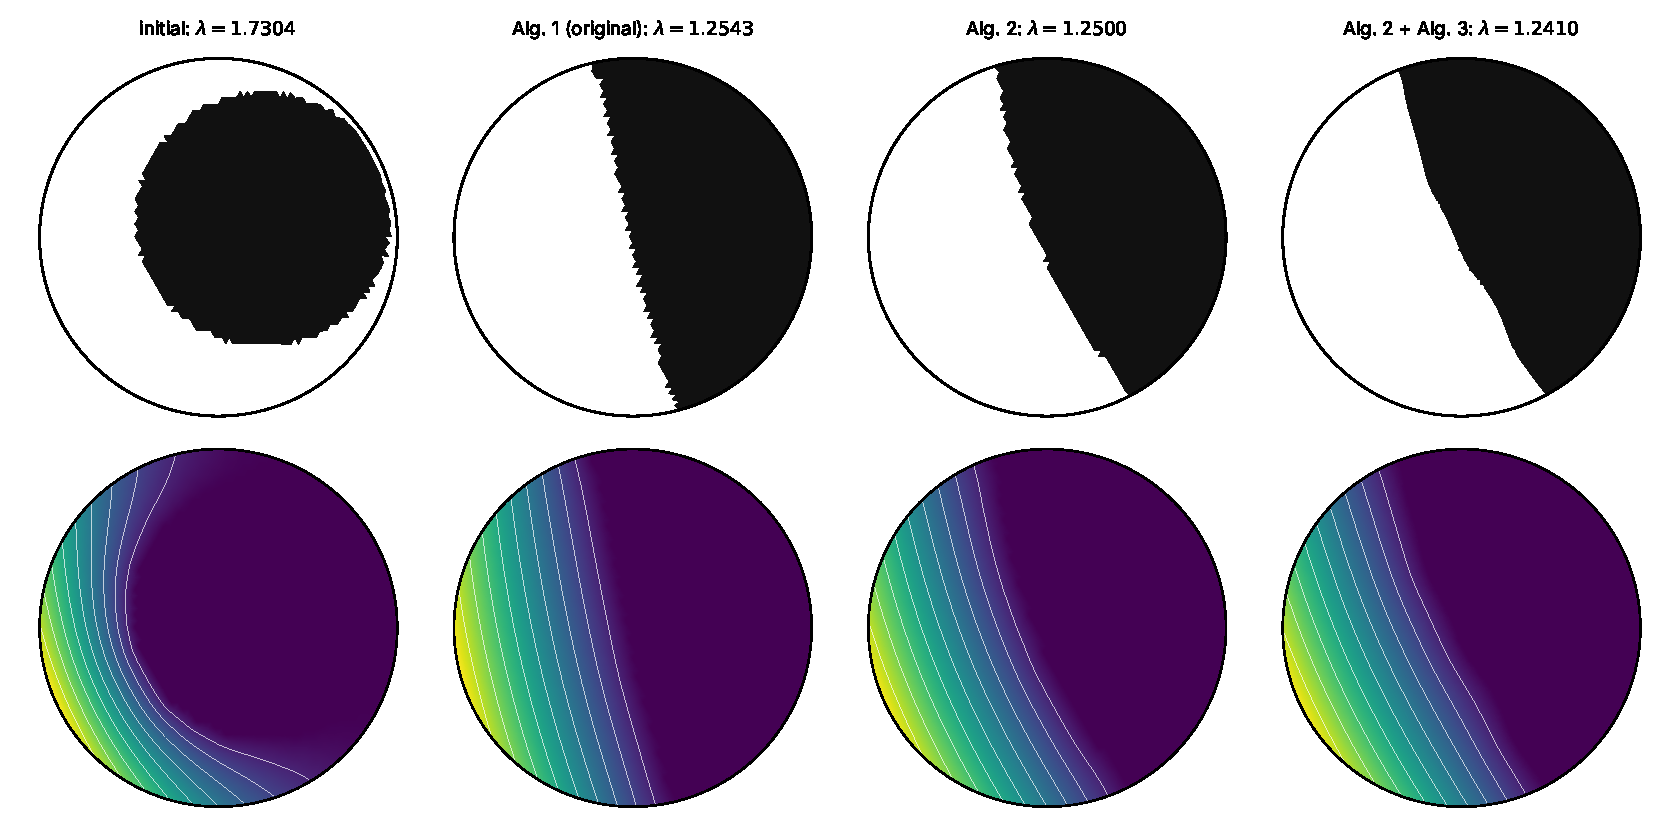
\includegraphics[width=\textwidth]{figures/holes_disk.pdf}
\caption{Unit disk, $\alpha=\pi/2$. From left to right: initial hole, Algorithm~\ref{alg.swap} and Algorithm~\ref{alg.rearr} started from it, and Algorithm~\ref{alg.flow} started from the output of Algorithm~\ref{alg.rearr}. The optimal hole touches $\partial\Omega$ on the side opposite to where the eigenfunction concentrates; it is neither the centered disk nor half of the disk (Theorem~\ref{t.ball}), and it is spherically symmetric, as predicted in \cite{FBRW1}.}\label{fig.disk}
\end{figure}

\begin{figure}[h]
\centering
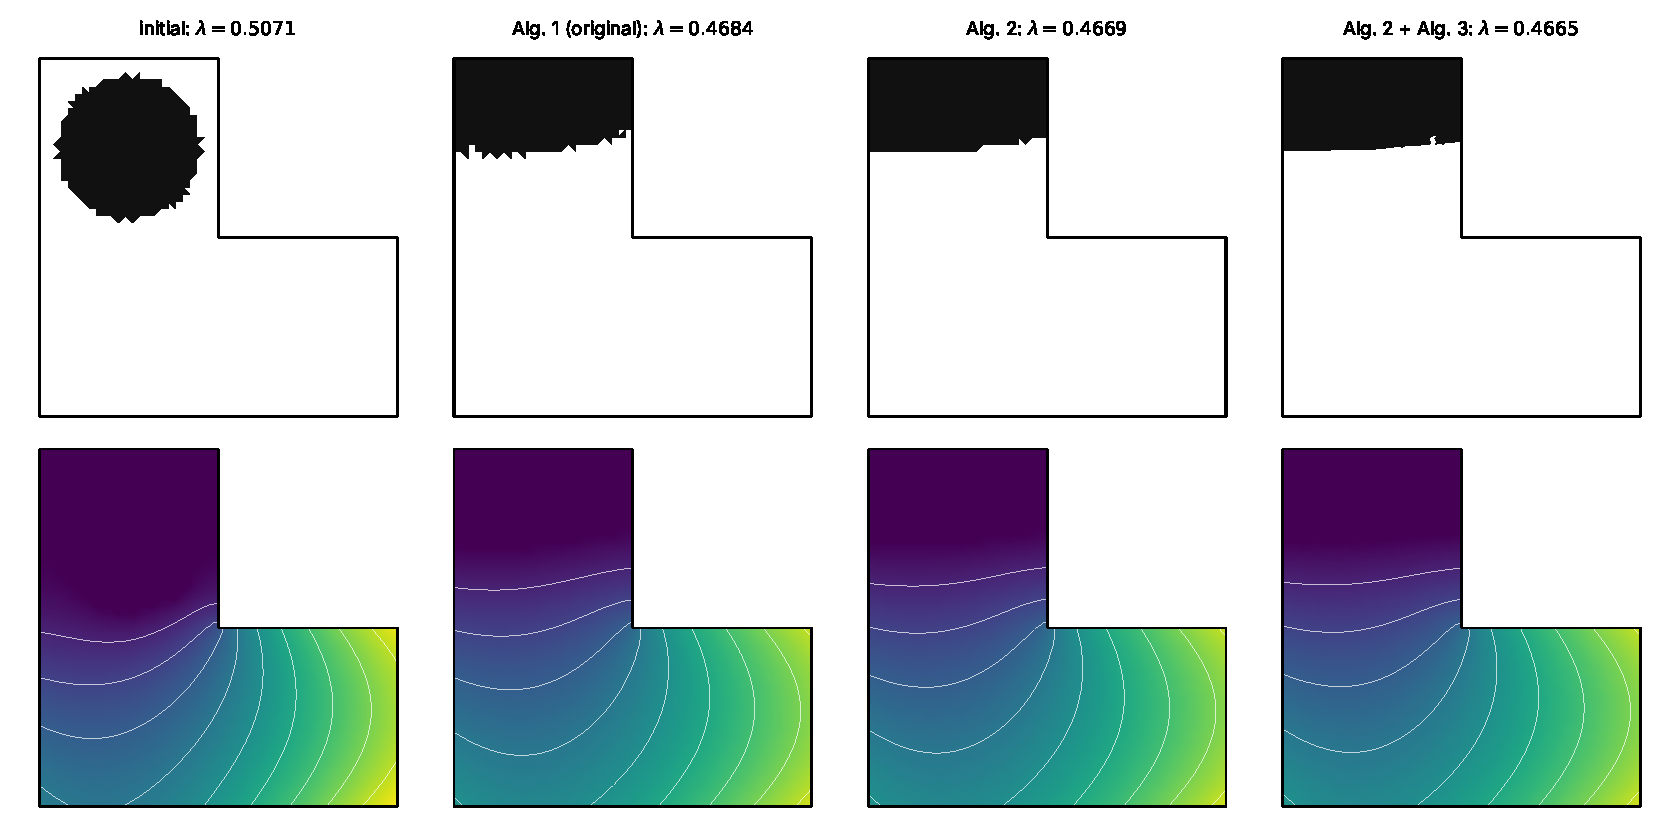
\includegraphics[width=\textwidth]{figures/holes_lshape.pdf}
\caption{L-shaped domain, $\alpha=1/2$. The optimal hole is a strip at the end of one of the two arms (by symmetry there are two optimal holes); Started in the corner square, both discrete algorithms stop at worse local configurations (Algorithm~\ref{alg.swap} at $0.506$, Algorithm~\ref{alg.rearr} at $0.577$); the figure shows the runs from an initial hole for which both find the strip.}\label{fig.lshape}
\end{figure}

\begin{figure}[h]
\centering
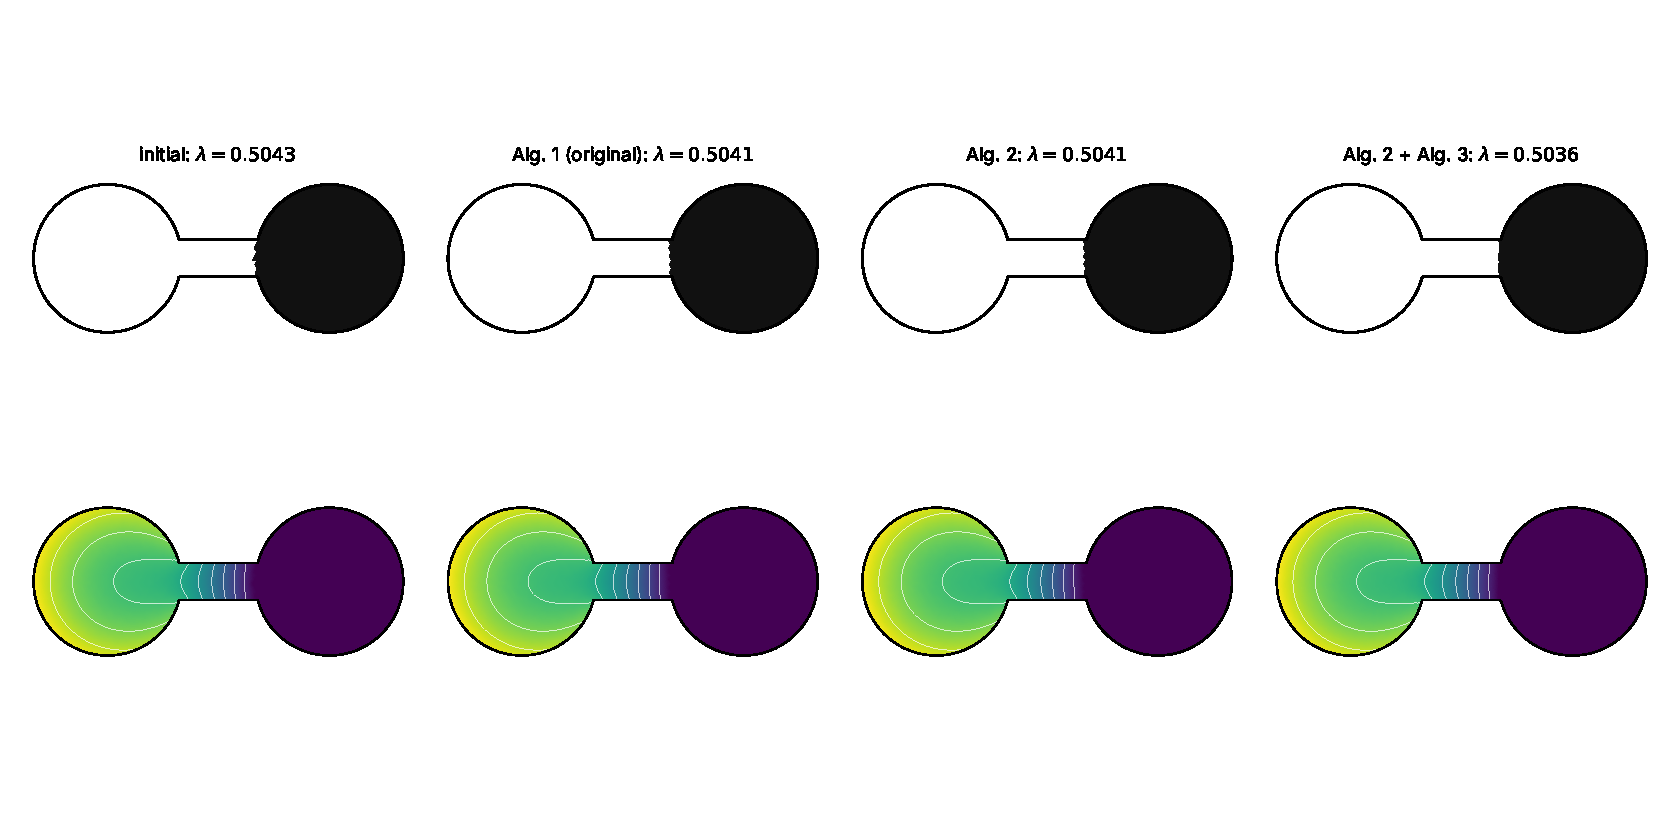
\includegraphics[width=\textwidth]{figures/holes_handle.pdf}
\caption{Two disks with a handle, $\alpha=\pi$: the optimal hole essentially fills one of the disks.}\label{fig.handle}
\end{figure}

\begin{figure}[h]
\centering
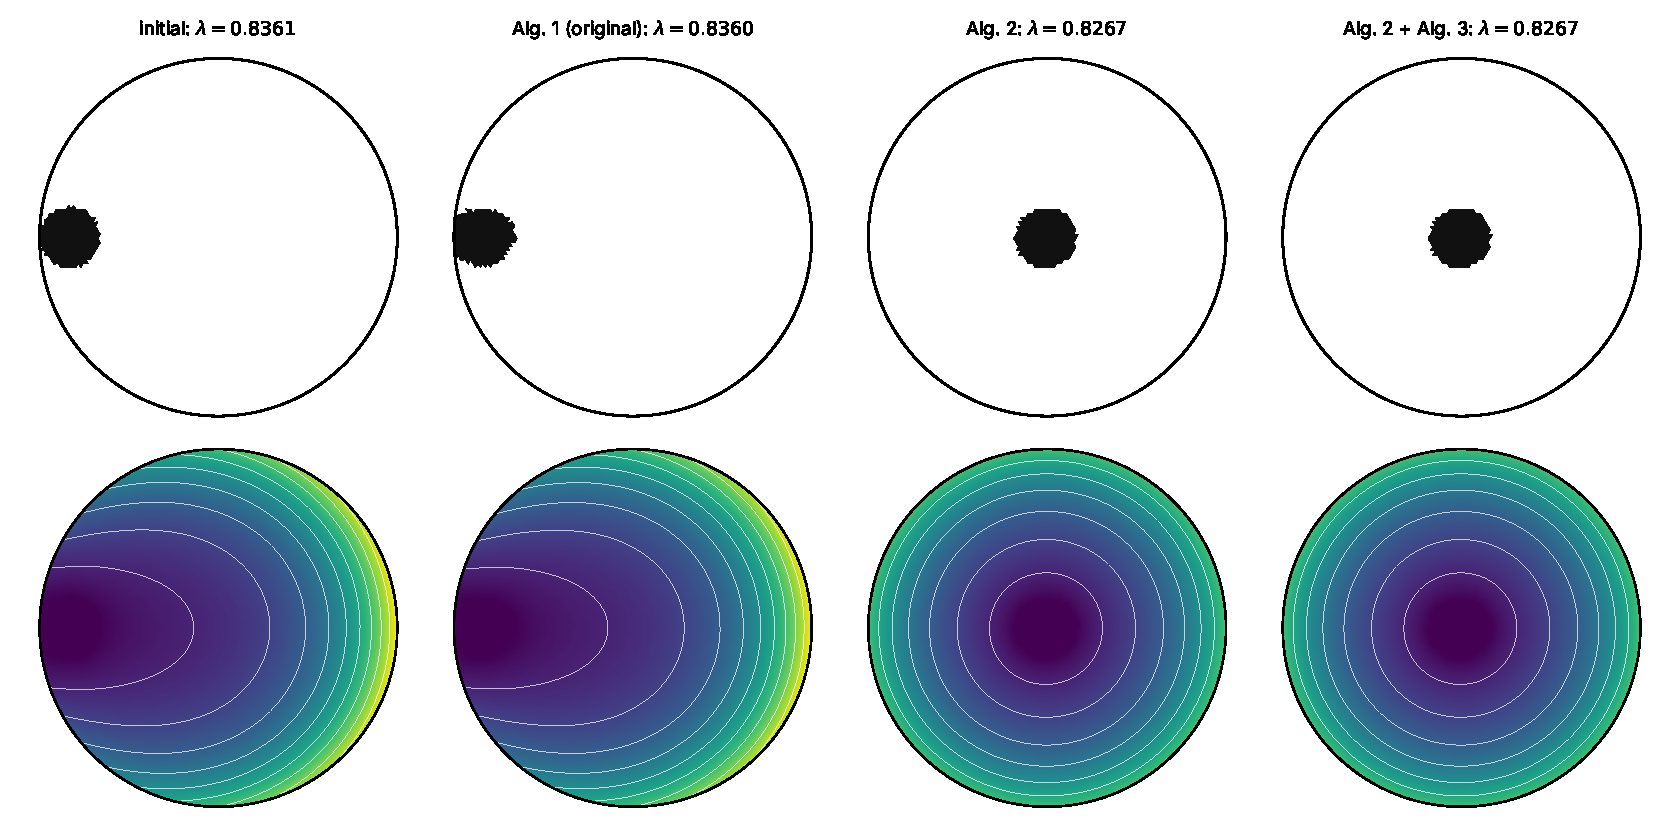
\includegraphics[width=\textwidth]{figures/holes_bigdisk.pdf}
\caption{Disk $B_3$, $\alpha=\pi/4$: here $R=3>R^*(0.5)\approx2.30$ and Algorithm~\ref{alg.rearr} converges to the centered disk from every initial hole (Conjecture~\ref{conj}); Algorithm~\ref{alg.swap} does too from the initial holes near the centre, but not, within 300 iterations, from a hole close to $\partial\Omega$.}\label{fig.bigdisk}
\end{figure}

\emph{Convergence as $h\to0$.} Table~\ref{tab.conv} and Figure~\ref{fig.conv} show the behavior of the computed optimal holes for the L-shaped domain with $\alpha=1$ (the example of Table~1 in the published version) as $h\to0$. The values of $\lambda_{1,h}$ decrease and stabilize, and the holes converge, in agreement with Theorem~\ref{t.fem}.

\begin{table}[h]
\centering\small
\begin{tabular}{rrrrrrr}
\hline
$h$ & nodes & $|A^*_h|$ & $\lambda_{1,h}$ (Alg.~\ref{alg.rearr}) & nodes & $|A_h|$ & $\lambda_{1,h}$ (Alg.~\ref{alg.flow})\\
\hline
0.2 & 96 & 1.0000 & 0.54588 & 206 & 0.9800 & 0.53282\\
0.1 & 341 & 1.0000 & 0.53713 & 525 & 0.9961 & 0.53188\\
0.05 & 1281 & 1.0012 & 0.53333 & 1766 & 0.9982 & 0.53122\\
0.025 & 4961 & 1.0000 & 0.53206 & 6259 & 0.9998 & 0.53079\\
\hline
\end{tabular}

\caption{L-shaped domain, $\alpha=1$: discrete optimal values obtained with Algorithm~\ref{alg.rearr} (structured mesh of size $h$, best of several initial holes) and Algorithm~\ref{alg.flow} ($h_{\rm fine}=h/2$). The deviation of $|A_h|$ from $\alpha$ is of order $h^2$, as expected for unions of triangles.}\label{tab.conv}
\end{table}

\begin{figure}[h]
\centering
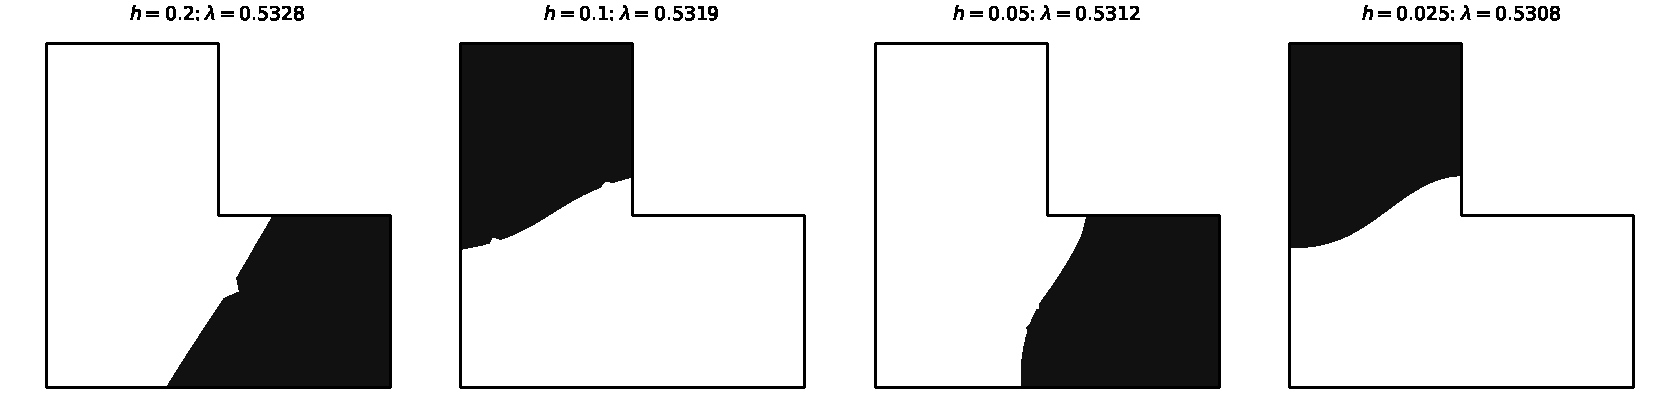
\includegraphics[width=\textwidth]{figures/convergence_lshape.pdf}
\caption{Optimal holes for the L-shaped domain with $\alpha=1$ as $h\to0$ (Algorithm~\ref{alg.flow}).}\label{fig.conv}
\end{figure}

\emph{The centered ball.} Table~\ref{tab.translation} and Figure~\ref{fig.translation} compare the second derivative of $\lambda_{1}(B_r(te_1))$ at $t=0$ given by \eqref{transl} with finite element computations on a conforming mesh of the annulus deformed by $x\mapsto x+t\eta(|x|)e_1$, with $\eta=1$ near the hole and $\eta=0$ near $\partial B_R$ (so that the mesh topology does not change with $t$). Figure~\ref{fig.regimes} shows the two regimes of Theorem~\ref{t.ball} in the $(r,R)$ plane.

\begin{table}[h]
\centering\small
\begin{tabular}{rrrrrrr}
\hline
$R$ & $r$ & $R^*(r)$ & $\lambda_1(R,r)$ & $\lambda_{1,h}(B_r)$ & $\frac{d^2}{dt^2}\lambda_1(B_r(te_1))|_{t=0}$ & FEM\\
\hline
1 & 0.2 & 1.6707 & 0.891127 & 0.891202 & $-1.738e+00$ & $-1.627e+00$\\
1 & 0.5 & 2.2994 & 1.608809 & 1.609044 & $-5.253e+01$ & $-3.304e+01$\\
3 & 0.5 & 2.2994 & 0.826216 & 0.826254 & $+1.220e-02$ & $+1.209e-02$\\
3 & 1 & 3.1159 & 0.852983 & 0.853019 & $-1.223e-02$ & $-1.147e-02$\\
5 & 0.5 & 2.2994 & 0.893693 & 0.893961 & $+3.462e-04$ & $+3.798e-04$\\
\hline
\end{tabular}

\caption{Translation of the centered hole ($N=2$): exact values from \eqref{explicit} and \eqref{transl} and finite element values.}\label{tab.translation}
\end{table}

\begin{figure}[h]
\centering
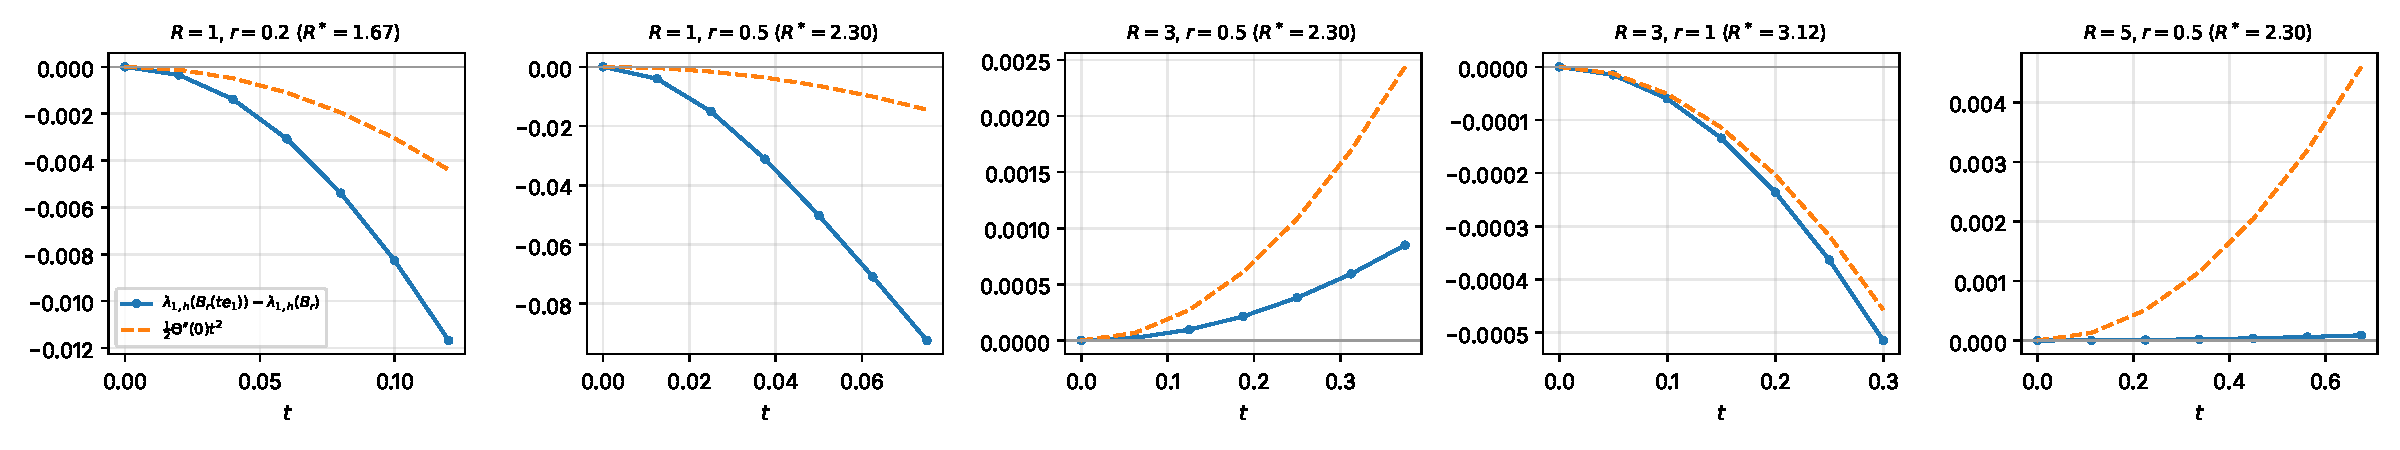
\includegraphics[width=\textwidth]{figures/translation.pdf}
\caption{$\lambda_{1,h}(B_r(te_1))-\lambda_{1,h}(B_r)$ (dots) and $\frac12\Theta''(0)t^2$ (dashed). For $R<R^*(r)$ the centered hole is a local maximum among translates; for $R>R^*(r)$ it is a local minimum. Note that $\Theta''(0)$ only bounds the true second derivative from above, but has the same sign (Proposition~\ref{p.second}).}\label{fig.translation}
\end{figure}

\begin{figure}[h]
\centering
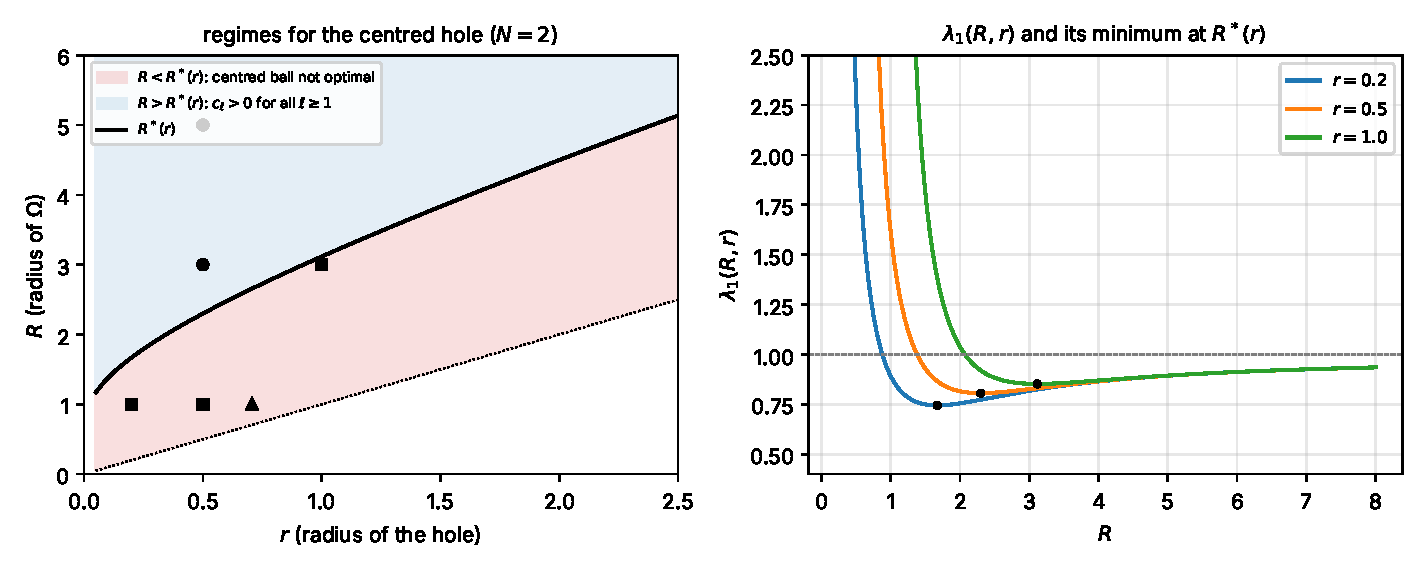
\includegraphics[width=\textwidth]{figures/regimes.pdf}
\caption{Left: the threshold $R^*(r)$ in the $(r,R)$ plane ($N=2$); squares: cases with $R<R^*(r)$; circles: $R>R^*(r)$; triangle: the unit disk with $\alpha=\pi/2$. Right: $\lambda_1(R,r)$ as a function of $R$ and its minimum at $R^*(r)$.}\label{fig.regimes}
\end{figure}

\subsection{Final comments}
Let us mention some difficulties and possible improvements.

The element-swapping algorithm (Algorithm~\ref{alg.swap}) may develop cycles, has many spurious minima (non optimal configurations such that removing any triangle of the hole and adding another one anywhere on its boundary increases the eigenvalue), is not monotone, and moves the interface by one layer of triangles per step; on the other hand, it is surprisingly robust with respect to the initial hole in some examples (the L-shaped domain). The rearrangement algorithm (Algorithm~\ref{alg.rearr}) is monotone for each $\beta$, converges in a few iterations, is several times faster and is able to change the topology of the hole in one step, but it is still a discrete method whose holes are unions of triangles, and it may stop at local minima. Since both discrete algorithms are cheap, running both from a few initial holes is a sensible strategy. The shape-gradient flow (Algorithm~\ref{alg.flow}) resolves the free boundary and its contact with $\partial\Omega$, with refinement near the interface, but it requires a good initial topology. The combination of a discrete algorithm (Algorithm~\ref{alg.rearr}, or both discrete algorithms) with Algorithm~\ref{alg.flow} is, in our experience, the most efficient strategy. Possible improvements include a second-order (Newton) step based on Proposition~\ref{p.second}, curvature-based regularization of the velocity, and the use of a level set representation of the hole.

As observed in the introduction, the measure of the discrete holes in Algorithms~\ref{alg.swap} and \ref{alg.rearr} satisfies $\alpha\le|A_h|\le\alpha+Ch^N$, since the triangles do not all have the same area; in Algorithm~\ref{alg.flow} the volume is corrected at each step and $||A_h|-\alpha|$ is of the order of the step size.

\subsection*{Acknowledgements}
We want to thank the anonymous referee for the careful reading of the manuscript, the constructive criticism and several suggestions that helped us to improve the paper.

\begin{thebibliography}{99}
\bibitem{Au} T. Aubin, Équations différentielles non linéaires et problème de Yamabe concernant la courbure scalaire. \emph{J. Math. Pures Appl.} \textbf{55} (1976), 269--296.
\bibitem{Bi} R. J. Biezuner, Best constants in Sobolev trace inequalities. \emph{Nonlinear Anal.} \textbf{54} (2003), 575--589.
\bibitem{CC} A. Cherkaev and E. Cherkaeva, Optimal design for uncertain loading condition. In: \emph{Homogenization}, 193--213, Ser. Adv. Math. Appl. Sci. 50, World Sci. Publishing, River Edge, NJ, 1999.
\bibitem{Ci} P. G. Ciarlet, \emph{The finite element method for elliptic problems}. North-Holland, Amsterdam, 1978.
\bibitem{DP} M. Dambrine and M. Pierre, About stability of equilibrium shapes. \emph{M2AN Math. Model. Numer. Anal.} \textbf{34} (2000), 811--834.
\bibitem{DH} O. Druet and E. Hebey, The AB program in geometric analysis: sharp Sobolev inequalities and related problems. \emph{Mem. Amer. Math. Soc.} \textbf{160} (2002), no.~761.
\bibitem{dPF} M. del Pino and C. Flores, Asymptotic behavior of best constants and extremals for trace embeddings in expanding domains. \emph{Comm. Partial Differential Equations} \textbf{26} (2001), no.~11-12, 2189--2210.
\bibitem{Es} J. F. Escobar, Sharp constant in a Sobolev trace inequality. \emph{Indiana Univ. Math. J.} \textbf{37} (1988), no.~3, 687--698.
\bibitem{FBLDR} J. Fernández Bonder, E. Lami Dozo and J. D. Rossi, Symmetry properties for the extremals of the Sobolev trace embedding. \emph{Ann. Inst. H. Poincaré Anal. Non Linéaire} \textbf{21} (2004), no.~6, 795--805.
\bibitem{FBR1} J. Fernández Bonder and J. D. Rossi, Asymptotic behavior of the best Sobolev trace constant in expanding and contracting domains. \emph{Commun. Pure Appl. Anal.} \textbf{1} (2002), no.~3, 359--378.
\bibitem{FBR2} J. Fernández Bonder and J. D. Rossi, On the existence of extremals for the Sobolev trace embedding theorem with critical exponent. \emph{Bull. London Math. Soc.} \textbf{37} (2005), no.~1, 119--125.
\bibitem{FBRW1} J. Fernández Bonder, J. D. Rossi and N. Wolanski, On the best Sobolev trace constant and extremals in domains with holes. \emph{Bull. Sci. Math.} \textbf{130} (2006), no.~7, 565--579.
\bibitem{FBRW2} J. Fernández Bonder, J. D. Rossi and N. Wolanski, Regularity of the free boundary in an optimization problem related to the best Sobolev trace constant. \emph{SIAM J. Control Optim.} \textbf{44} (2006), no.~5, 1614--1635.
\bibitem{Fl} M. Flucher, \emph{Variational problems with concentration}. Progress in Nonlinear Differential Equations and their Applications 36, Birkhäuser, Basel, 1999.
\bibitem{He} A. Henrot, Minimization problems for eigenvalues of the Laplacian. \emph{J. Evol. Equ.} \textbf{3} (2003), no.~3, 443--461.
\bibitem{HP} A. Henrot and M. Pierre, \emph{Variation et optimisation de formes. Une analyse géométrique}. Mathématiques \& Applications 48, Springer, Berlin, 2005.
\bibitem{Ka} T. Kato, \emph{Perturbation theory for linear operators}. Classics in Mathematics, Springer, Berlin, 1995.
\bibitem{KS} C.-Y. Kao and S. Su, Efficient rearrangement algorithms for shape optimization on elliptic eigenvalue problems. \emph{J. Sci. Comput.} \textbf{54} (2013), 492--512.
\bibitem{LDT} E. Lami Dozo and O. Torné, Symmetry and symmetry breaking for minimizers in the trace inequality. \emph{Commun. Contemp. Math.}, to appear.
\bibitem{LZ} Y. Li and M. Zhu, Sharp Sobolev trace inequalities on Riemannian manifolds with boundaries. \emph{Comm. Pure Appl. Math.} \textbf{50} (1997), 449--487.
\bibitem{MR} S. Martínez and J. D. Rossi, Isolation and simplicity for the first eigenvalue of the $p$-Laplacian with a nonlinear boundary condition. \emph{Abstr. Appl. Anal.} \textbf{7} (2002), no.~5, 287--293.
\bibitem{PS} P.-O. Persson and G. Strang, A simple mesh generator in MATLAB. \emph{SIAM Rev.} \textbf{46} (2004), no.~2, 329--345.
\bibitem{Pi} O. Pironneau, \emph{Optimal shape design for elliptic systems}. Springer, 1984.
\bibitem{Re} W. Reichel, Radial symmetry for elliptic boundary-value problems on exterior domains. \emph{Arch. Rational Mech. Anal.} \textbf{137} (1997), 381--394.
\bibitem{Sc} L. Schwartz, \emph{Cours d'analyse}. 1 et 2. Second edition, Hermann, Paris, 1981.
\bibitem{Sp} E. Sperner, Spherical symmetrization and eigenvalue estimates. \emph{Math. Z.} \textbf{176} (1981), 75--86.
\bibitem{St} M. W. Steklov, Sur les problèmes fondamentaux en physique mathématique. \emph{Ann. Sci. École Norm. Sup.} \textbf{19} (1902), 455--490.
\end{thebibliography}

\end{document}
